

\chapter{Background}
\label{sec:sota}
\minitoc
\bigskip


% INTRO (nico): Definir le pbm de la locomotion. 
% Ses specificites et difficultes: system instabable + grande dimension + divergence exponentielle mise en evidence par le charriot-sur-la-table, nature discrete des contacts conduisant a une dynamique hybride, robustesse.
% Noter l'objectif de l'equipe, dans lequel tu t'inscrits: obtenir des methodes realistes qu'on puisse mettre en oeuvre sur le robot reel. Lien avec le CG et la biomech

% New intro sota by nico
Our contribution in this thesis aims at addressing the very complexity of the locomotion problem, where the decision on continuous motion variables and discrete contact locations have to be taken from an intricate process.
The study of this problem started more than 50 years now, with very quickly the ambition of getting a complete solution, i.e. a complete motion controller driving the locomotion of real robots, and later on, dynamic avatars evolving in physical simulation subject to realistic constraints.

In this chapter, we will first browse the various approaches that have been historically proposed, until recent locomotion controllers able to optimize or learn all degrees of freedom at once (Section \ref{sota1}).
This will help us understanding the key aspect of locomotion: the intricated decision of motion and contact.
We will then focus on one subpart of the locomotion problem: contact planning (Section \ref{sota2}). In this thesis, we will be interested in one particular approach to tackle this problem called motion-before-contact, that we will argue to be promising for the main realistic locomotion problems, that we will connect to the navigation problem.
In Section \ref{sota3}, we will list the main existing solution to navigate in a 3D environment with legged system.
Finally, we will conclude the chapter by defining our thesis propositions and explaining how they contribute to the state of the art.


% ==== THE MAIN PROBLEM =====
% (P1+P2+P3) Too hard, too many dimensions, we do not know how to do.
% => Need contact planning.
% For dynamic walking, this is often done at the same time than the WBC because it's difficult to approximate it (hybrid solution), but for quasi-static it's ok.
% (P1+P2) How to do, it is a combinatorial problems. Some people like DEITS use a MIP or simplify the problem, others use a guide alleviate the combinatorics.
% (P1) We use some path planning algorithms (sampling-based) but a problem comes that is the feasibility of the guide with P2. We have some heuristics built empirically but overall, we do not know how to do.
% => Use Reinforcement Learning to learn how to do it.

% ==== Other problem ====
% Path planning is long to compute + the steering are often not terrain-aware, there are some works on navigation that could be helpful.

% ==== PLAN ====
% (P3 => P2)
% Explain the works on locomotion (P3) 
% Why we need contact planners (P2)
% Separate in two: 
% - contact-before-motion (most of the works)
% - motion-before-contact
% => P1
% In P1, there is path planning that have been searched extensively

\section{Synthesizing Locomotion \label{sota1}}
%\href{}{Link}\\
% Read well the related work of Ewen + RLOC
% P3 directly, on flat ok, on uneven we do not know (too big dim), lot of collisions, not suitable for biped. We need to specify the footstep location. (most works are in graphics for that, PPO paper etc). Then most of them relies on pre-defined footsteps to work.

% WBC aims to i) define a small set of simple, low-dimensional rules (e.g., equilibrium, self-collision avoidance, etc.) ii) that are sufficient to guarantee the correct execution of any single task, whenever feasible (e.g., reaching for an object with one end-effector), and of simultaneous multiple tasks (e.g., reaching for an object with one end-effector, while reaching for a second object with another end-effector), iii) exploiting the full capabilities of the entire body of redundant, floating-based robots in compliant multi-contact interaction with the environment.

% NICO SAYS BLABLA
%Locomotion of legged characters is a long-searched but still challenging topic.
%During its motion, the robot is constantly subject to dynamic constraints such as maintaining its equilibrium or avoiding collision of its body with the environment and itself.
%Its motion also has to be coordinated to perform a given task such as walking in a given direction or moving its feet to the next desired placement.
%The robot motion is performed by the \textit{whole body controllers}, which are among the most difficult controllers to engineer due to their numerous stability criteria \cite{Chevallereau_book, kajita_intro_humanoid_robotics}.

%In this section we classify the whole body controllers in two categories, namely \textit{contact agnostic} and \textit{contact-based} approaches.
%First, we review some contact agnostic works, that do not require (nor plan) the next contacts to perform with the environment. Those approaches have seen a lot of success recently with the use of RL algorithms for character locomotion.
%We then explore more classical and predominant contact-based approaches in the literature. 
%Those use predefined contact sequences or plan contacts with the environment during the motion simultaneously.

% Remarques nico:
% Definir le titre, methodes locales des premiers controlleurs de loco, fondees sur des lois de controle ou sur des principes d'optimalite permettant d'en obtenir.
% En quoi peut-on/doit-on les separer d'algo "planif" => Pas de recherche explicite de contact, eventuellement comme effet de bord du mouvement corps complet?
% Preciser: double grille de lecture
% - critere 1: decision de contact (imposee, guidee, libre, implicite)
% - Conformite du modele (Template LIPM, reduit, complet)
% Nous on choisit le critere 1 pour l'organisation des sections.

Research on modeling legged robot movements for locomotion is a long searched topic \cite{history_humanoid_robots}.
The task of determining stable and feasible motions is performed by the \textit{whole body controllers} (i.e. controller able to take real-time decisions about all the robot degrees of freedom whole body). They are among the most difficult controllers to engineer due to their numerous stability criteria \cite{chevallereau_book, kajita_intro_humanoid_robotics}.


% nico:
We propose here to explore these methods by first obtaining a complete movement on the real robot in a realistic simulator.
This exploration will help us understanding the importance of planning the future contact of the system in its environment.
As we will see, while contact planning can initially be considered aside from the whole body controller, recent advances tend to more effectively consider both problems together
%\textcolor{blue}{Nicolas veut ajouter une footnote (voir latex en dessous), mais je suis vraiment pas sur que ca apporte quelque chose}
%\footnote{While we acknowledge the completeness of the unified (contact+whole body) locomotion problem, we will argue in Section \Section{sota2} of properly handling the contact planning problem, both for immediate practical resolution and future fundamental understanding of the geometrical complexity it brings to the full locomotion problem}.

We will browse through the panel of existing locomotion controllers, that we can explore following 2 criteria:
\begin{description}
   \item[(1) Contact decision,] that can be predefined, internal, or free.
   \item[(2) Model complexity,] if the model is templated (e.g. Linear inverted pendulum model), reduced, or complete.
\end{description}
%This section is organized following criterion (1) based on the contact decision.
%We will use both with their respective importance.

\subsection{Predefined Contacts}
\begin{figure}[h]
    \centering
    \captionsetup[subfigure]{justification=centering}
    \begin{subfigure}[t]{0.4\linewidth}
    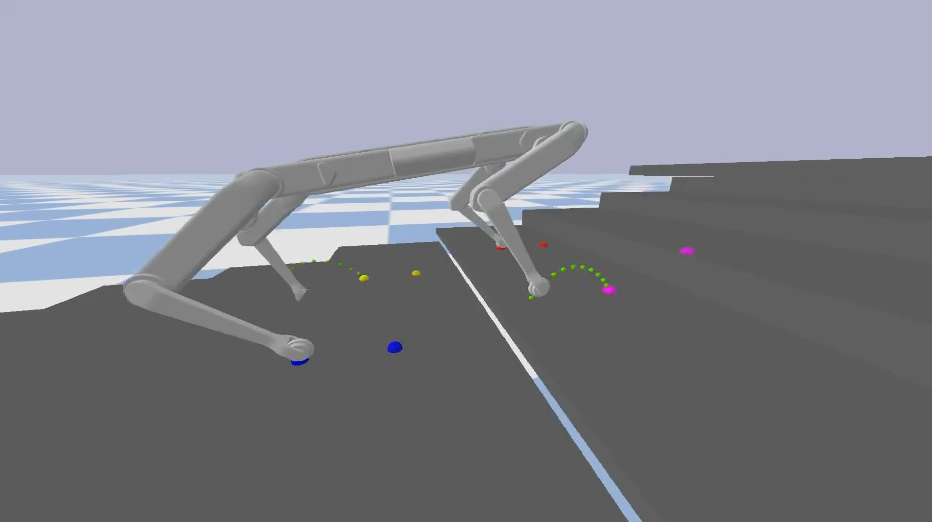
\includegraphics[width=\textwidth,height=4cm]{Figures/Chapter_SOTA//fanny_corbere_solo.png}
    \caption{Risbourg et al. \cite{fanny_mip_solo}}
    \label{fig:mpc_predefined_0}
    \end{subfigure}
    \begin{subfigure}[t]{0.58\linewidth}
    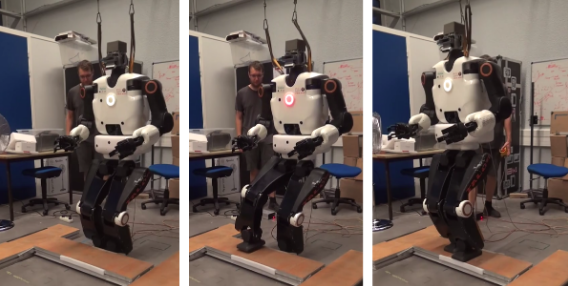
\includegraphics[width=\textwidth,height=4cm]{Figures/Chapter_SOTA//talos_ewen.png}
    \caption{Dantec et al. \cite{ewen_2022}}
    \label{fig:mpc_predefined_1}
    \end{subfigure}
    \label{fig:mpc_predefined}
    \caption{Whole body controllers performing predefined contacts.}
\end{figure}
Given a predefined contact sequence, efficient methods exist to compute the corresponding stable whole-body motion.
% Dynamics / Quasi-static
Knowing the dynamic state of the robot (e.g. position and velocity of its basis and all its joints) as well as its current and future contacts, approximation models can be used to plan the whole-body locomotion of legged characters.

\paragraph{Model-based approaches.}
Due to the high complexity of the locomotion problem, classical whole-body controllers of this category often rely on simplified dynamic robot models.
% LIPM
In the seminal work, Kajita et al. \cite{kajita2003ZMP} introduced some key methods of the robot locomotion field: the linear inverse pendulum and the zero moment point.
This contribution is the basis of numerous works based mainly on the study of the centroidal dynamics for walking robots \cite{Tonneau2018_2PAC, caron_2018_whole_body}.
Given a contact sequence, some Model-Predictive Control (MPC) methods permit to compute a trajectory for the robot center of mass, while ensuring its dynamics consistency \cite{carpentier2016_versatile_efficient, pierre_alexandre_2021}.
% IK
From the simplified model estimations, a whole body motion can then be generated over a short horizon, following it as a reference \cite{felix_and_avadesh_2019}.
Carpentier et al. \cite{loco3d} use a second-order inverse kinematic to follow a reference centroidal trajectory, previously generated by their optimization method.
Also, the inverse kinematics can be used to compute collision-free robot motion, such as Risbourg et al. \cite{fanny_mip_solo} who adapt the end-effector trajectory of the quadruped robot SOLO to avoid its collision with the environment (Figure \ref{fig:mpc_predefined_0}). %\cite{CHOMP_2009, stomp_2011, schulman_2014_collision, perrin_2012, fanny_mip_solo}
% Autre comme ewen
Alternatively, other approaches exist to achieve all in one whole body MPC. Dantec et al. \cite{ewen_2022} propose such an MPC taking into account the whole body model to achieve dynamic locomotion on the torque-controlled humanoid robot Talos over predefined footsteps (\ref{fig:mpc_predefined_1}). Their control directly computes the optimal torque to be applied on the robot without any additional trajectory or estimation.



\paragraph{Learning whole-body controllers.}
Such whole-body controllers can also be learned by reinforcement in simulation \cite{ALLSTEPS_2020}.
Peng et al. \cite{deepLoco} train a biped character in simulation to follow predefined footsteps, and achieve walking in mostly flat environments.
Following this idea, Tsounis et al. \cite{deepGait} learn a whole-body controller in simulation for quadruped locomotion on more complex terrains. 
Gangapurwala et al. \cite{RLOC} learn whole-body motion tracking and recovery controllers for improved robustness, accounting for changes in the dynamics of the robot and perturbations. Their policy is then performed on a real quadruped robot.
Combining model-based and RL approaches, Xie et al. \cite{glide_xie_2021} learn by reinforcement how to control the accelerations of a centroidal model, then used to compute ground reaction forces translated to joint torques applied on the robot.
Their method, combined with simple heuristics for footstep placement, demonstrates robust walking in complex scenes on the quadruped robot Laikago. %\textcolor{blue}{Is glide set in the right section ? For me yes.}

To this day, such controllers are mostly applied in the real-world to quadruped robots and have yet to be performed on humanoid robots \cite{papier_rohan_wbc_rl_2022}.

\paragraph{Conclusion on predefined contacts.}
Most of the works in the literature focus on whole-body controllers generating motions over predefined contact sequences.
Model-based approaches have shown impressive locomotion skills on complex environments \cite{ladder_robot_2}.
Reinforcement learning is another approach to obtain such controllers. 
The trained controllers can cope with the system dynamics along with stability criteria. 
However, they require up to several days of training, and are yet to achieve the results of model-based controllers on real humanoid robots.

In this thesis, we will be using Task-Space Inverse Dynamics (TSID)-based controllers \cite{tsid_prete}, following the methodology introduced in the context of the Loco3D project \cite{loco3d}, yet expecting the coming generation of robot controllers to be rather base on whole body MPC \cite{ewen_2022}.
In the meantime, we explored RL-based controllers.
While we can hope that future discoveries will lead to the unification of these different concepts, all are indeed compatible with the approach discussed in this thesis.
We will explore in Section \cite{sota2} that what really matters is to characterize their feasibility domain. 
%\textcolor{blue}{I do not talk about it in sec 2, let's see if it changes.}

\subsection{Internal Contact Decision}
%\textcolor{blue}{Avant "Explicit contact decision", j'aime pas trop le terme parce qu'au dessus c'est aussi explicite. Si c'est calcule en interne par le WBC... j'ai mis internal?}
\begin{figure}[h]
    \centering
    \captionsetup[subfigure]{justification=centering}
    \begin{subfigure}[t]{0.30\linewidth}
    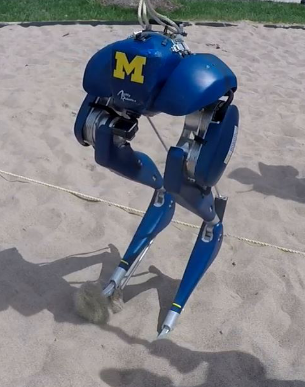
\includegraphics[width=\textwidth,height=4.5cm]{Figures/Chapter_SOTA//cassie_walking_sand.png}
    \caption{Gong et al. \cite{Cassie_feedback_control_2018}\label{fig:walking_task_0}}
    \end{subfigure}
    \begin{subfigure}[t]{0.45\linewidth}
    %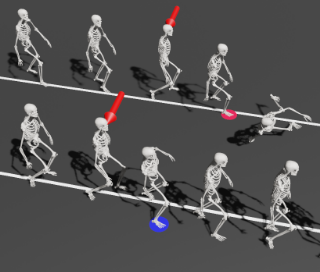
\includegraphics[width=\textwidth,height=4.5cm]{Figures/Chapter_SOTA//hwangpil_biped_stability.png}
    %\caption{Park et al. \cite{hwangpil_stable_2020} }
    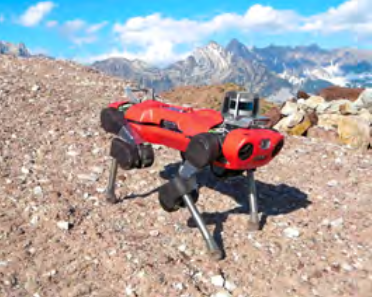
\includegraphics[width=\textwidth,height=4.5cm]{Figures/Chapter_SOTA//anymal.png}
    \caption{Lee et al. \cite{hutter_challenging_terrain}\label{fig:walking_task_1}}
    \end{subfigure}
    \caption{Legged robots walking on small variation terrains.\label{fig:walking_task}}
\end{figure}

%Whole-body controllers can also compute the contacts internally along with the robot motion.

\paragraph{Flat floor.}
%\textcolor{blue}{To modify?}
Traditional whole-body controllers for flat ground locomotion make the assumption that contacts will always occur at the same height in global space.
Achieving stable, periodic walking on flat ground is already a challenging problem in itself to comprehend the nature of dynamic models for locomotion, which is especially difficult for biped robots \cite{grizzle_chevallereau_2010}.
The study of the center of mass trajectory, with the linear inverted pendulum model and zero moment point as well as their variations, has been at the core of the legged locomotion problem with model-based approaches \cite{zmp_history, Wieber2016, carpentier_thesis_2017}.

%\textcolor{blue}{What I say bellow for chevallereau + tsujita has to be rechecked. I am not confident in this part on model-based WBC.}
A common strategy to solve this problem is to use a reference walking motion, which is then modified by the whole-body controller to ensure its stability at runtime.
Using such a controller, Chevallereau et al. \cite{Chevallereau_2008_zmp} modify the reference joint motion to obtain the desired zero moment point evolution, and thus a stable walking motion.
%modify a reference motion in order to ensure a stable motion. (e.g. model predictive control), mostly using the so called Zero Moment Point (ZMP) \cite{zmp_history}, and low level controller tracking this reference motion (e.g. feedback control).
Tsujita et al. \cite{gait_pattern_2001} propose a gait pattern controller adapting the reference motion in function of touch sensor signals on the foot of a quadruped robot. % They use a non-linear oscillator to have a nominal ref motion that is modified in function of the touch sensors.

% Using simplified models (as winkler 2018 says)
Simplified models of robot dynamics are an effective strategy.
Using a linear inverted pendulum as a reduced model of the robot, Kajita et al. \cite{kajita2002LIP2} propose a real-time walking pattern generator that adapts footsteps during the motion to follow a desired walking speed and direction.
% They optimize CoM - CoP - Footstep simultaneously.
In this line of work, Herdt et al. \cite{herd_2010, herd_perrin_2010} introduce the notion of \qq{walking without thinking}, where a model predictive control scheme takes as input a given direction to follow, and outputs safe foot placements and motion to walk seamlessly while reacting to disturbances on the humanoid robots HRP2.
% Other task inside the MPC => Footstep plan in function
Such a strategy permits fast online planning \cite{hurst_2018} as well as the optimization of different tasks simultaneously such as locomotion and manipulation \cite{florent2012} or obstacle-avoidance in real-time \cite{naveau2017}.
%However, these approaches are mostly limited to flat grounds due to their formulation.
%A limitation of these controllers is that they are by nature short horizon planner that would be prone to local minima on more complex scenarios (where the robot motion gets trapped in a loop and is not able to go forward). \textcolor{blue}{Is my definition ok or I'm totally wrong}


\paragraph{Small variation terrains.\label{par:whole-body:uneven}}
%Another strategy is to consider a nominal reference motion on flat ground, then make it robust enough to be performed on complex terrains.
This strategy naturally extends when the motion on flat ground is robust enough to be performed on complex terrains.
It can be done by simplifying the robot dynamics model with templated models to generate a nominal reference motion considering a flat ground.
This motion is then performed by the whole body controller that adapts it for complex and rough terrains.
Rezazadeh et al. \cite{rezazadeh_hurst_atrias_2020} include a reflex-based control scheme to walk blindly on uneven terrain with the biped robot Atrias.
Building upon this work, Gong et al. \cite{Cassie_feedback_control_2018} adapt motions from a gait library and demonstrate various locomotion tasks on the biped robot Cassie including   balancing on uneven moving surfaces or walking in the sand (Figure \ref{fig:walking_task_0}).

In computer graphics, learning a controller from data can produce natural and plausible walking motion \cite{learned_motion_matching, pfnn}.
However, data-driven strategies often require a large amount of motion capture data, and cannot cope with the dynamics variations in the robot (or character) states inherent to physics-based simulations and the real world.

Reinforcement learning, and more specifically imitation learning, can overcome this limitation and bridge the gap between simulation and reality (sim-to-real).
Li et al. \cite{CassieLi2021} learn to adapt motion from a gait library. 
They then achieve the sim-to-real by randomizing the system dynamics in simulation, and achieve robust locomotion on the biped robot Cassie.
% Hutter => Quadruped in the nature.
Using another strategy, Lee et al. \cite{hutter_challenging_terrain} learn a teacher policy for walking on the quadruped robot ANYmal, that is fully aware of its surrounding environment.
The safe motion generated by the teacher is then imitated by another policy, that learns how to blindly walk in complex terrains.
They then demonstrate walking in the real world in very rough scenarios (Figure \ref{fig:walking_task_1}).
% Residual
Learning residual control is another method to bridge the reality gap. Duan et al. directly learn how to modify the reference motion with residual actions to obtain a more robust bipedal walking \cite{residual_rl_cassie_2021}.

While these works demonstrated some capabilities to walk in uneven terrains, they remain limited in more complex scenarios. 
Indeed, such "blind" controllers are performing a control only in reaction to impacts on the environment. They are on the opposite anticipating proper contact creation, or briefly taking advantage of more advanced knowledge about their environment. As a consequence, they are irremediably prone to collisions (and falls) on terrains such as stairs.

\paragraph{Simultaneous motion and contact optimization.\label{par:simul_contact_motion}}
%\stn{reprends la structure du sota du journal de daeun, elle est tres bien pour differencier les 2. Tu dois surtout expliquer la logique. Le truc clef c est pas la taille du modele. C est de dire on smooth un pb discret en un probleme continu. Les papiers se situent par rapport a cette frontiere. Tu dois mettre ca en chapeau. Les premiers papiers en ont pas besoin parce qu hyothese simpificatrice, les autres si. Donc c est ca ta distinction: comment tu formule le contact de maniere continu. Soit en reduisant l espace de recherche, soit en lissant la dynamique}
%\textcolor{blue}{Je suis dans la section des whole body controller. Parler de la difference entre continue/discrete approches pour la selection des surfaces/contacts n'est peut etre pas le bon endroit?}

Optimizing simultaneously contact and motion permits the consideration of the robot dynamics in the contact choice, considering a known terrain model.

% It's planning => offline and long, but this time we can consider the terrain and optimize everything.
% Mordatch 2012
% Carlos 2017
% Carlos 2020
% Winkler + hutter 2018 (MIP for the whole stuff)
% Ponton 2020 (same on SOLO, check the diff)
Approximating the environment as a continuous function and computing contact and motion permits the generation of whole-body motion in complex terrains \cite{Dai_2014, posa2014}.
In simulation, Mordatch et al \cite{mordatch2012DiscCIopt} present a contact invariant method optimizing contacts and motion trajectory simultaneously to perform a wide variety of locomotion tasks.
In the same line of work, Winkler et al \cite{winkler2018GaitOpt} present a trajectory optimization formulation generating highly dynamic motion plans for a variety of legged characters on complex terrains.
Whole-body trajectory optimization was successfully applied to real quadruped robots, achieving planning on flat ground and execution of walking movements in near real-time \cite{Winkler2017_TO}.

%Mixed Integer Programming (MIP) formulation can be used to solve the discrete choice of the next contact surface selection and continuous optimization of the motion, extending this method for quadruped locomotion to uneven terrains \cite{carlos_2019}.

%Trajectory optimization of simplified or full dynamics model is promising to perform safe and robust locomotion, benefiting from the contact-based approach as well as considering the dynamic state of the robot in the planning as well as the terrain constraints.
%However, as the size of the model used and the complexity of the terrain increase, this approach suffers from high computation time (up to several seconds per footstep), limiting its application for real-time planning. 
%Some promising works solve this limitation \cite{ponton_righetti_2020, hutter_last_work_nmpc}, but they rely on a separate planner to find the next contact surface to step on.

The key aspect of these approaches is to consider some piecewise-smooth representation of the contact variables. The contact sequence can then evolve continuously on a piecewise-smooth world while the motion solver explores various locomotion patterns, in a continuous (optimization-based) manner. Of course, this prevents some world representations such as Mario-style floating platforms, yet not reducing much the applicative scope. 
The main limitation comes from the inability of the (convex) optimization solver to handle the non-convex nature of the contact location in a non-flat world. 
Moreover, this also prevents the solver to discover non-regular gaits, or with some clever but non generic reformulation \cite{winkler2018GaitOpt}.


On the other hand, it has been proposed to explicitly model the discrete nature of the contact sequence by integer variables, hence leading to an optimization problem deciding of a mix of continuous and discrete variables, called Mixed-Integer Programming (MIP) \cite{gurobi_mip}.
With this approach, Aceituno-Cabezas et al. simultaneously optimize contact, gait and motion planner on their quadruped robot on complex terrains \cite{carlos_2019}.
However, MIP does not scale well to these large or non-linear problems, hence reducing up to now the impact of these approaches to whole body problems.
On the other hand, this limitation can be solved if we can keep a linear formulation \cite{sl1m_v1}. This approach will be further covered in this thesis.

 %\textcolor{red}{On the other hand, MIP solver are very efficient algorithm if we can keep a linear formulation (SL1M). In this thesis, we will capitalize on this approach and show how we can exploit it to generate whole body movements, by connecting it to the notion of feasibility.}

\paragraph{Conclusion on internal contact decision.}
A classical approach for locomotion is to synthesize walking motion while adapting footstep placement on flat ground.
Generalizing these approaches to uneven terrains is feasible but limited, as such controllers consider the terrain variations as errors during the motion that needs to be fixed.
%Finally, trajectory optimization is promising to plan safe walking motion on complex terrains. However, these methods are still expensive to compute.
For more complex scenarios, numerical solvers fail to globalize the exploration and discover interesting locomotion patterns.
We better understand the complexity of the search when explicitly formulating it as a MIP problem, then boiling down to a combinatorial exploration.

\subsection{Contact Agnostic}
Whole-body controllers previously presented implicitly or explicitly reason about contact placement on the terrain.
Another strategy is to employ a contact agnostic approach, where the controllers are not given any reference motion or contact sequence.
%, and are provided with little to no info about the terrain.
The contact sequence is then not an explicit variable, but rather a consequence of the whole-body actions, often locally based on its surrounding environment knowledge.

%They have to answer the following question: \textit{can we generate walking motion without reasoning about contact placements on the terrain?}

%These approaches typically uses sensor datas of the robot to estimate its stability.
%Previous works presented in Section \ref{par:whole-body:uneven} answers the question considering a walking motion on flat ground and relying on the robustness of their whole-body controller to adapt to more complex terrains. However, the expected walking motion implies to reason about contact placement to a certain extension.

%This section is an informational overview of works on locomotion with a contact agnostic approach.

\paragraph{Optimal control with differentiable simulation.}

When optimizing the robot trajectory with fixed contact sequence, the reason why the solver cannot decide to change the sequence is that the contact dynamics are set as non-differentiable. 
Indeed, in robotics and computer graphics, we often consider rigid (stiff) contact solvers, which offer the best trade-off between algorithmic efficiency and realism \cite{pybullet_coumans2019}.
Yet this leads to non-differentiable models that gradient-based algorithms cannot manipulate. 
In \cite{hamalainen_2015} a gradient-free solver is used on top of the rigid (ODE) simulator, leading to contact exploration even if with a local exploration range.
%On the other hand, a smooth relaxation of the stiff contact dynamics \cite{mujoco} also leads to contact discovery, again with local capabilities.

In order to use gradient-based algorithms, finite-differencing can typically be used to approximate the gradients such as the physics engine MuJoCo \cite{mujoco}. However, it tends to introduce round-off and discretization errors.
Recently, some differentiable physics engines have emerged to solve these issues, such as Nimble from Werling et al. supporting complex contact geometry and gradients approximating continuous-time elastic collision \cite{werling_2021}.
So far, this direction has not been pushed to a realistic robot setup. 
Current works are mostly on the simulator formulation \cite{chainqueen_2019, difftaichi_2019} or on local smoothing using randomization \cite{tedrake_2022_differentiable, carpentier_fix_differentiable_OC}.



\paragraph{Learning how to locomote.}
\begin{figure}[h]
    \centering
    \captionsetup[subfigure]{justification=centering}
    \begin{subfigure}[t]{0.36\linewidth}
    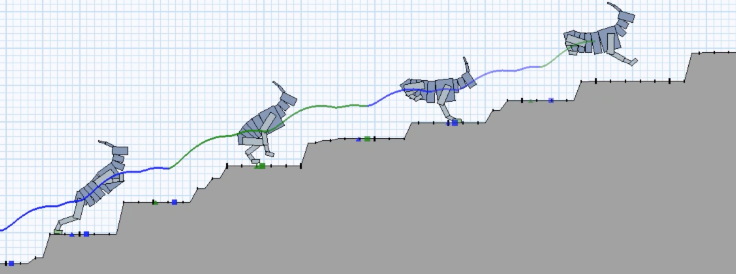
\includegraphics[width=\textwidth,height=3cm]{Figures/Chapter_SOTA//terrain_adaptive.png}
    \caption{Peng et al. \cite{terrain_adaptative_locomotion}}
    \label{fig:rl_agnostic_0}
    \end{subfigure}
    \begin{subfigure}[t]{0.36\linewidth}
    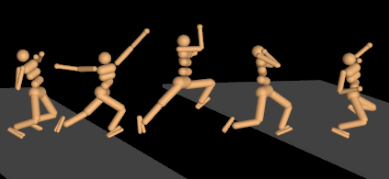
\includegraphics[width=\textwidth,height=3cm]{Figures/Chapter_SOTA//deepMindPPO.png}
    \caption{Heess et al. \cite{ppo_rich_locomotion} }
    \label{fig:rl_agnostic_1}
    \end{subfigure}
    \begin{subfigure}[t]{0.25\linewidth}
    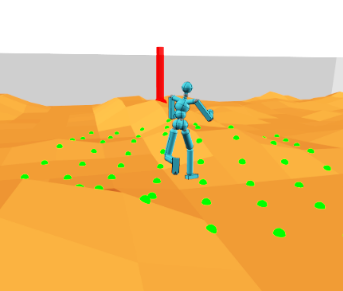
\includegraphics[width=\textwidth,height=3cm]{Figures/Chapter_SOTA//vae2.png}
    \caption{Won et al. \cite{VAE_jungdam_2022}}
    \label{fig:rl_agnostic_2}
    \end{subfigure}
    \label{fig:rl_agnostic}
    \caption{Works on reinforcement learning for legged characters locomotion.}
\end{figure}

Similarly to trajectory optimization, Reinforcement learning can explore movements to optimize an objective function. Yet they offer unprecedented flexibility in environments and the objective they can tackle. Furthermore, they only require optimization at training time, while the run-time only consists of the execution of the resulting policy.
% PETTRE SURVEY: RL stands out as a promising approach for character animation because it provides a versatile framework to learn motor skills without the need of labelled data. RL is particularly useful when the dynamic equations of the environment are unknown or non-differentiable, to which conventional gradient-based optimal control algorithms do not apply.
As they do not require the evaluation of the simulator gradients, they are also less prone to the limitations discussed with trajectory-based solvers related to contact differentiability, and accept classical (stiff) contact formulation.


% That is where Reinforcement Learning becomes really useful in physics-based sim.
Reinforcement Learning (RL) in physics-based simulation can be used for character animation \cite{survey_rl_animation_pettre_2022}.
This method permits learning controllers able to cope with the system dynamics.
%They offer better generalization capabilities to new environments or unexpected events compared to traditional model-based approaches that are highly complex to engineer. 
Peng et al. learn by reinforcement a terrain-adaptive locomotion controller, outputting target joint angles to compute the torques on 2D biped and quadruped characters \cite{terrain_adaptative_locomotion} (Figure \ref{fig:rl_agnostic_0}). 
Using a similar control, such RL controller can be extended to 3D locomotion \cite{ppo_rich_locomotion} (Figure \ref{fig:rl_agnostic_1}).
%for example using Proximal Policy Optimization (PPO) RL algorithm \cite{PPO_2017}.
These seminal works are the basis of many others further improving the naturalness and robustness of the motions as well as the diversity of skills performed \cite{drecon, carl, Lee_muscles_rl_2019}.
More recently, Won et al. \cite{VAE_jungdam_2022} use conditional variational autoencoders to learn how to imitate motion from a database and achieve various tasks in a physics-based simulation. 
One of their results shows a biped locomotion task using a low-resolution local height map as terrain observation to walk and run on rough terrains.

Evolutionary algorithms can be a suitable alternative to RL, even to learn locomotion skills from scratch \cite{evol_vs_rl_deepmind_2017}. 
While both approaches present their pros and cons \cite{evol_vs_rl_majid_2021}, they also present similarities as they both learn from interactions with the environment.
Covariance matrix adaptation is one evolution strategy that can be used to learn walking by controlling torques \cite{yin_simbicon_2007, wang2009} or musculo-tendon units on humanoid characters \cite{wang2012} and various biped creatures \cite{van_de_panne_2013}.

% Mini conclusion
The recent breakthroughs in RL algorithms such as PPO \cite{PPO_2017} and others \cite{TD3_2018, SAC_2018} have permitted the learning of highly adaptive whole-body controllers on rough terrains for legged character locomotion in simulation.
% Very promising alternative to model-based, but not very stable
These methods are promising to compensate for the weaknesses of model-based approaches, which can be difficult to develop and demonstrate fewer generalization capabilities.
However, these controllers are often long to train as they require millions of interactions with the environment. Moreover, the motions generated are usually jerky visually, and the search for a more stable bipedal walk with RL remains \cite{hwangpil_stable_2020}.
%Finally, some works show that acting in task space (e.g. proportional derivative control) \cite{does_choice_action_space_peng_2016} and leveraging the knowledge of traditional model-based controllers is promising to learn controllers faster, while producing more robust behaviors.

\paragraph{Robot learning and sim-to-real.}
% But as said previously, the fidelity of the simulation compared to the real world is not good.
Several works using RL demonstrate how to learn to walk on legged characters in simulation.
However as stated in the survey of Ibarz et al. \cite{survey_sergey_robot_rl}, a policy learned in simulation usually performs badly on the real robot due to the discrepancy between the simulation and the real world.

% Sim-to-real methods
Diverse sim-to-real methods have appeared to bridge the reality gap such as randomizing the simulation dynamics \cite{peng_domain_randomization_2017}, identifying the dynamics parameters on the real robot \cite{liu_sim_to_real_2019} or developing an accurate actuator model and simulating latency \cite{sim_to_real_agile_2018}.
% This has been moved to Uneven terrains.
%Li et al. \cite{CassieLi2021} randomize the dynamics of the system in the simulation using \cite{peng_domain_randomization_2017} and learn to imitate motions from a gait library in simulation, to then achieve robust locomotion on a real biped robot.
% Hutter => Quadruped in the nature.
%Lee et al. \cite{hutter_challenging_terrain} learn a teacher policy fully aware of the robot surrounding environment to teach another policy how to perform a robust blind quadrupedal locomotion in simulation, then demonstrate walking in very rough scenarios (Figure \ref{fig:rl_agnostic_robot_1}).
While those methods alleviate the reality gap problem, they do not compensate totally for the environment model inaccuracy in simulation. 
That is why such trained controllers could require additional fine-tuning on the real robot.

Despite some recent success, the sim-to-real transfer is mostly a matter of robustness, that we can now improve at the cost of longer training and less optimality. One of the stakes in reinforcement learning is to rather adapt the learning to the real robot dynamics.




\paragraph{Robot learning in the real world.}
\begin{figure}[t]
    \centering
    \captionsetup[subfigure]{justification=centering}
    \begin{subfigure}[t]{0.48\linewidth}
    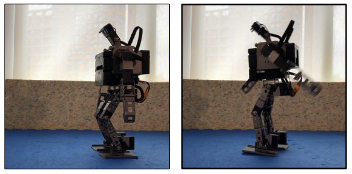
\includegraphics[width=\textwidth,height=4cm]{Figures/Chapter_SOTA//heess_robot.png}
    \caption{Bloesch et al. \cite{rl_wild_heess_2022}}
    \label{fig:rl_agnostic_robot_0}
    \end{subfigure}
    \begin{subfigure}[t]{0.4\linewidth}
    %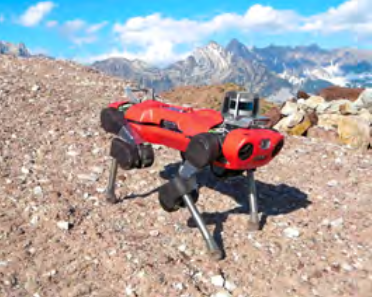
\includegraphics[width=\textwidth,height=4cm]{Figures/Chapter_SOTA//anymal.png}
    %\caption{Lee et al. \cite{hutter_challenging_terrain}\label{fig:rl_agnostic_robot_1}}
    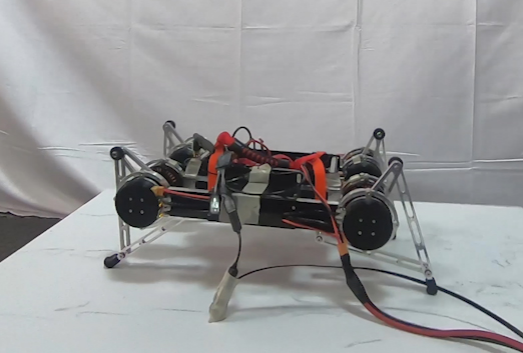
\includegraphics[width=\textwidth,height=4cm]{Figures/Chapter_SOTA//sergey_rl.png}
    \caption{Haarnoja et al. \cite{sergey_2018}}
    \label{fig:rl_agnostic_robot_1}
    \end{subfigure}
    \caption{Robots learning how to walk in the real world.}
    \label{fig:rl_agnostic_robot}
\end{figure}
% What's the challenge in robotics
% We do not want to break the robot => No collision if possible, no strong impacts, jerky movements lead to dynamics instability making the robot fall or collide so we need to avoid it.
Learning controllers by reinforcement directly on real robots is a appealing direction to remove the dependency on imperfect simulation \cite{rl_robotics_survey_2013}.
However, such an approach is challenging due to critical real-world limitations.

The sampling collection is a tedious process on the real robot, and so the policy has to be learned from a significantly less amount of data. As a consequence, algorithms with better sample efficiency are required \cite{sergey_2018, calinon_micro_rl}.

Reinforcement learning algorithms are trial-and-error processes, thus leading to numerous failures during learning. 
In the real world, these failures translate into a high risk of breaking the robot and a potential threat to the safety of its surroundings.
% Some attempts to learn directly on the real robot with RL (spider etc).
As a result, learning whole body controllers \qq{in the wild} \cite{rl_wild_heess_2022}, meaning directly on the real robot, requires additional safety measures.
% Talk first about RL directly on the robot: quadruped (Sergey Levine 2019) + Towards General and Autonomous Learning (Hafner 2020)
Most works on the topic avoid such an issue by learning on relatively small-sized and harmless robots \cite{nao_rl_world_docking, rl_wild_heess_2022}. 
Back in 2005, Tedrake et al. learned how to walk by reinforcement directly on a low degree of freedom biped robot \cite{tedrake2005learning}. 
Later on, as the RL algorithms and robot designs improved, learning locomotion from scratch has been performed on quadruped \cite{sergey_2018} (Figure \ref{fig:rl_agnostic_robot_1}), hexapod \cite{deepmind_locomotion_RL} and more complex biped robot \cite{rl_wild_heess_2022} (Figure \ref{fig:rl_agnostic_robot_0}).
Another limitation of learning in the real world is that during the training (up to several hours or days), the human will have to manually reset the robot position as it falls over, bumps into a wall, or reaches the edge of the terrain.
% Safety: recovery policy (Tan 2022)
Yang et al. \cite{yang2022safe} alleviate this limitation by lowering the number of falls. They propose a safe recovery policy to take over the control when the learning agent violates some safety constraints, thus decreasing the need for human intervention while improving the safety of the robot.
% Previously in the other chapter
Finally, some strategies can use knowledge from a simulation to quickly learn how to adapt to the real world.
% Mouret with robot that can adapt like animal => Hard to place
With a small hexapod robot, Mouret et al. \cite{Mouret_adapt_like_animals_2014} learn in simulation a behavior map using evolutionary algorithms, then composed of thousands of walking behaviors. At runtime on the real robot, this map can be efficiently searched using optimization algorithms. 
Their results demonstrate that the robot can learn to select the best walking behavior among this map in a few trials, to compensate for its body damage and to adapt to its environment.

% But it's long and high risk to break the robot => Still a research topics and not feasible at all on biped for now.
Applying RL in the wild is an exciting research direction. But it is for now limited in the context of locomotion to small robots that require constant human intervention during training, and which has only been applied to flat ground so far.
Designing bigger-sized robust robots or strategies to make the robot automatically recover \cite{leo_robot_2010} are promising directions.

\paragraph{Conclusion on contact agnostic approaches.}
%Classical model-based controllers have been extensively studied over the past years to achieve blind walking \cite{Cassie_feedback_control_2018}.
%However, those are complex to engineer as they require some good models of the robot and dynamics, and can lack the ability to adapt to unexpected variations in the environment due to their constant uncertainty about the position of the next contact. 
% So the safest way is to learn in simulation then pass it in simulation => Sim-to-real problem.
The recent surge in the use of reinforcement learning has proven promising to develop controllers with a contact agnostic approach.
Works on this topic demonstrated impressive results to generate robust walking motion, while adapting to the rough terrains in simulation \cite{VAE_jungdam_2022} and in the real world \cite{yang2022safe}.

Nowadays, learning robot locomotion (and other skills) in the wild is yet limited to small robots for safety and cost reasons.
Learning from simulation remains the best way to ensure the safety of the robot and its surroundings.
It also permits to easily reset the robot state, and bypass the poor data efficiency of learning on real systems \cite{atrias_rl_sim_to_real} (i.e. tedious collection process of data). 
However, learning safe and robust walking on biped robots without specifying a reference motion or contacts is still difficult.
Finally, the search for more accurate simulations or efficient sim-to-real methods remains.

%Furthermore, contact agnostic approaches are inherently limited due to their blind nature which irremediably leads to a high number of collisions in more complex environments as well as potentially strong impacts on the terrain.
%These limitations put at risk the robot and its surrounding, which we cannot afford on costly big-sized robots.


\subsection{Conclusion}
% Conclusion: On a des methodes qui existent pour generer le whole body motion pour des pas donnees (s'ils sont faisables). D'autres methodes essaient de generer ou replannifier ces pas en meme temps que le whole body motion, mais ont des temps de calcul vraiment enorme ce qui n'est pas possible pour du online-replannning sur le vrai robot. 
% Comme on veut un temps de calcul rapide <<1mn, on doit donc utiliser des pas predefinis en amont de la whole body locomotion, c'est a dire faire du Contact Planning. 
% Cette hierarchical decomposition rend le probleme plus facile a traiter.

%Whole body controllers with a contact agnostic approach are complex to engineer. 
%Their blind nature allows them to detect contacts with the terrains only after the impact. In spite of few successes with traditional model-based and more recently RL controllers, they remain limited to low variations grounds and cannot be applied to more complex terrains without guarantee of safety for the robot. \textcolor{blue}{Safety may not be the right word?}
% Say that it's blur
%It is important to note that contact agnostic controllers still consider contact placements to some extent. 
%Indeed, a blind controller will somehow expect the next contact to be at a fixed position on flat ground and adapt as best its control in function of its sensors measurement.

%Accurately defining contact position is essential to obtain a stable and safe locomotion behavior.
%Methods optimizing the motion and the contact position simultaneously permit to obtain of dynamic motions, but are not yet real-time capable due to the high dimension of the problem solved.
%Whole-body controllers to perform a predefined sequence of footsteps have been extensively studied in the literature, and several of them do this task efficiently \cite{carpentier2016_versatile_efficient, pierre_alexandre_2021, ewen_2022}.

%In order to get a safe and fast to compute locomotion planner, working with predefined contacts remains the most efficient strategy.
%Now we are left with one question: \textit{How to obtain these contacts ?}
%Manually defining those is a solution for fixed scenarios, but to obtain a more general locomotion planner we need to investigate the so-called \textit{contact planning problem}.

% Nicolas: 
% Real interest for contact agnostic, but not feasible yet.
% Explicit contact decision: limited to flat ground, and when applied to more complex terrains => Not stable/collision or too expensive to compute.
% As a result, to fastest and prefered solution to generate a walking motion is still to rely on a prior contact decision. This contact sequence can be given by the user, but we desire to automatize this task. So we have to see the contact planning.

In summary, we can classify the existing locomotion controllers in 3 categories, whether they cannot decide the contact variables, or explicitly optimize them as continuous or partly discrete values, or agnostically decide the contacts as a consequence of the movements.

%Contact decision is thus still required to generate a safe and robust walking motion.
Implicitly optimizing the contact position along with the motion is mostly limited to flat ground scenarios.
While recent whole-body controllers can demonstrate good generalization to uneven terrains, they are still inherently limited due to their blind nature.
Simultaneous motion and contact optimization are promising to generate dynamic and safe locomotion. 
However, they remain expensive to compute, thus limiting their use for online planning.

Research in locomotion has seen a lot of interest in contact agnostic approaches using reinforcement learning.
However, these methods are not mature yet to be feasible on a real human-sized robot.


%Following predefined contacts is still the most efficient way to synthesize locomotion. 
%To that end, efficient whole-body controllers exist to perform this task \cite{carpentier2016_versatile_efficient, pierre_alexandre_2021, ewen_2022}.

For now, all these methods fail to properly generalize to some kind of complexity in the locomotion scenarios (e.g. handrail grasping), to the more unstable bipeds, or to efficient robot deployment.
In general, the best strategy in all these cases is to rely on an external algorithm to decide or guide the contact decision \cite{carpentier2016_versatile_efficient, pierre_alexandre_2021, ewen_2022}.

Now we are left with one question: \textit{How to obtain these contacts ?}
Manually defining them is a solution for fixed scenarios, but to obtain a more general locomotion planner we need to investigate the so-called \textit{contact planning problem}.


% ===============================================================================


\section{The Contact Planning Problem \label{sota2}}

% Was made a nice choice because of the improvements in approx of feasiblity (CROC) for example.

% - 2 - Contact planning
% We need to plan contact for biped locomotion. The decoupling of whole body motion and footstep planning is faster but raise another problem that is the feasibility of the plan by the WBC, all mostly solved by the state of the art contact planners available. Separated in two families:
% Contact-before-motion: most of the works with many different strategies. Consist in searching the best foosteps to perform among all surfaces, subject to a combinatorial problem when planning several steps ahead.
% Motion-before-contact: A lot less know, consists in computing a rough root trajectory for the root of the robot (motion) before computing the contacts relative to this trajectory. This method constraints the exploration of the combinatorics of the contact planning only along this root trajectory, alleviating the combinatorics probem.

A contact planner finds a discrete sequence of contact positions that the robot has to perform to go through the terrain.
It is expected that the produced contact sequence does not come with a complete whole body trajectory, although some of its elements may be computed as well depending on the underlying algorithm.

%\textcolor{blue}{Nico dit d'ajouter une figure? Voir si j'en trouve une.}
As stated by Chestnutt et al. \cite{chestnutt_2009_interactive_guide}, planning footsteps rather than whole body motion allows the robot to reason about contact with the environment to ensure safe and stable support. This also reduces the planning state space to a dimensionality computationally tractable for online walking.
From a sequence of predefined contacts, efficient whole body controllers exist for motion planning \cite{carpentier2016_versatile_efficient, caron_2018_whole_body, pierre_alexandre_2021, ewen_2022}.
The division of whole-body control and contact planning greatly lowers the complexity of the locomotion problem. Indeed, it relies on simplifications and assumptions on the robot dynamics to efficiently compute a feasible sequence of contacts.
However, it also comes at the cost of the non-guarantee of the feasibility of the contact plans. 

The question of feasibility is of the main importance here, as we will show in this section: given a contact sequence in a given environment, can we guarantee that there exists a corresponding whole-body trajectory that follows it? 
This feasibility question is irrelevant for the previously presented methods which compute motion and contacts simultaneously \cite{Winkler2017_TO, carlos_2019}.

In this section, we classify contact planners of the literature into two categories as described by Bretl et al. \cite{bretl2006}:
\begin{itemize}
    \item \textit{contact-before-motion}, that decides the future contact placements, before planning the whole body motion.
    \item \textit{motion-before-contact}, that further divides the contact planning into two sub-problems. First plan a rough trajectory the robot root has to follow, which we call the \textit{guide path}, then compute the contact placement along it, and finally the whole-body motion.
\end{itemize}
We will explore the results of both strategies, along with their pros and cons.

\subsection{Contact-before-motion\label{subsub:contact-before-motion}}
\begin{figure}[ht]
    \centering
    \captionsetup[subfigure]{justification=centering}
    \begin{subfigure}[t]{0.48\linewidth}
    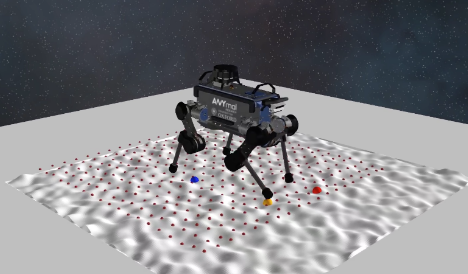
\includegraphics[width=\textwidth,height=4cm]{Figures/Chapter_SOTA//rloc_planning.png}
    \caption{Gangapurwala et al. \cite{RLOC}}
    \label{fig:cp_bm_0}
    \end{subfigure}
    \begin{subfigure}[t]{0.48\linewidth}
    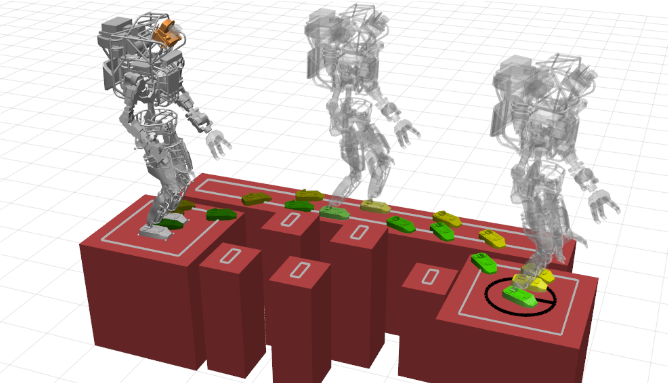
\includegraphics[width=\textwidth,height=4cm]{Figures/Chapter_SOTA//MIP_deits.png}
    \caption{Deits et al. \cite{deits2014FootPlanMI}}
    \label{fig:cp_bm_1}
    \end{subfigure}
    \label{fig:cp_bm}
    \caption{Contact-before-motion strategy with (a) short horizon and (b) long horizon planning.}
\end{figure}

%\textcolor{blue}{Fanny proposait de mettre cette section apres: Expliquer d'abord comment on place les contacts, ensuite comment on verifie s'ils sont valides. Moi je propose l'inverse, comment on verifie si un contact est valide, et ensuite comment a partir de ca on planifie. Quel ordre serait le mieux?} 
%\stn{a ce stade le schema de ma these aurait vraiment ete utilise qqe part}
Planning contact placements prior to the whole-body motion raises a key problem: \textit{how to know if a sequence of contacts is feasible by the robot?}
A naive positive proof would be to exhibit the corresponding whole body trajectory. However, we would need a cheaper decision test, which ideally should also prove a negative answer.
% Explanation
Seminal works solve this question using simplified models of the robot dynamics in its environment. Their related concepts such as the zero momentum point \cite{kajita2003ZMP} or contact wrench cones \cite{trinkle_2002_cwc} can be used to characterize the stability of contact configurations. 
Assuming quasi-static locomotion is also a classic assumption that simplifies the contact planning problem with approximated stability criteria. With this approach, we can plan robust contact placements that the robot can follow while staying in static equilibrium during the single and double support phases \cite{prete_static_equilibrium_2016}.
%where the robot could potentially stand above in static equilibrium during its contact transition . %but leading to unnatural and slow motions.
However, a quasi-static approach also limits the contact planners as they consider slow enough and in constant equilibrium motions. %\textcolor{blue}{Need reformulation?} 
Recently, computing the dynamic transition feasibility to a next contact has been made efficiently \cite{CROC} and allows for more dynamic locomotion. %\textcolor{blue}{Need to be reformulated?}

Finally, we need to answer the question: \textit{where to place these contacts in the environment?}
For that, we will explore contact planners operating at two different scales, short-horizon and long-horizon planning.

% Short horizon
\paragraph{Short horizon planning.}
% No combinatorial involved when computing the contacts on a very short horizon:
This approach focuses on computing the immediate next contact (or few contacts) to be performed by the robot, following a given direction.

As one could guess, this approach is particularly fast to compute as it is often based on simple heuristics for foot placement while respecting equilibrium and environment constraints \cite{raibert_heuritics_1986}.
Using this strategy, Scianca et al. \cite{Scianca_2020} compute the next footstep to be made on flat ground, then adapt and perform it by their whole-body controller on the humanoid robots NAO and HRP-4.
% Rebulla at darpa => problem of local minima highlighted.
Rebulla et al. \cite{rebula_2007_little_dog} present a model-based controller for quadruped robots planning only the next footstep to statically walk on rough terrains.

Reinforcement learning has also been used to choose the next few contact positions to be performed by the robot \cite{deepGait, RLOC} (Figure \ref{fig:cp_bm_0}). However, they often require complex reward design, long learning time (tens of hours), and the learned policies are specific to each robot model.

% These works provide very short horizon footstep planners, that are not subject to the combinatorics but can lead to local minima, where we are not sure of the feasibility of the future planning, where the choice of a footstep can lead to a deadlock.
Short horizon contact planners are fast to compute (a few milliseconds per step) but are by definition not designed for global planning, as they cannot guarantee its completeness to reach a distant goal. 
%\textcolor{blue}{I do not know if it's clear.} \stn{le pb c est pas l optimum global c est est ce qu on va se casser la figure}
Indeed, they are likely to navigate to insurmountable obstacles in complex environments, thus leading to local minima.
However, those characteristics make them particularly suited for robot locomotion with joypad-like user guidance to avoid unfeasible scenarios.

% Interrogation
%A relevant question one could ask: \textit{are there any benefits in computing only the next footstep placement, over methods planning footstep and motion simultaneously presented in Section \ref{par:contact_motion}?}
%On the one hand, planning both simultaneously can offer more dynamic motion, while offering some real-time planning on flat ground \cite{Winkler2017_TO} but not yet on complex scenes (order of seconds to plan a few steps).
%On the other hand, the division of both tasks clearly shows its benefits on the computation time and as a result, planning contact before whole-body motion remains to this day the most efficient method for online replanning in complex environments. \textcolor{blue}{To keep/remove/modify ?} 
%\stn{ca va pas. C est pas la dynamique le pb, c est l espace de recherche. Tu peux avoir un truc trs dynamique a un pas, mais avec un comportement myopique atteindre de mauvais minima. Je capte pas pourquoi tu opposes ça a winkler. Quand tu galeres comme ca fais une liste a item pour contre, voire un tableau. D ailleurs je pense resumer les contribs majeure dans un tableau me semble clef. tu prends 10 papiers et tu coches les proprietes}

\paragraph{Long horizon planning.}
% Question: is there a reason for planning several footsteps ahead ? If a solution exist, searching the combinatorics is more likely to find it rather than short horizon planners.
This approach solves a global contact planning problem in order to reach a distant goal. 
%In most cases, an infinity of contact placement combinations potentially exists to perform this task.
Of course, as, we have no means to know in advance the number of required steps for that, it often leads to long discrete sequences of decisions with potential underlying combinatorics.
As a consequence, contact planning on a long horizon is a combinatorial problem that takes longer to solve, but that should offer guarantees of optimality and completeness (i.e. it must find a solution if one exists) given enough computation time.
% On longer horizon planning (i.e. to reach a distant target), the combinatorics can be solved in several ways.
We identify two approaches in the literature to solve this problem: discrete and continuous.
% The most common in the litterature are discrete approaches using a path planning algorithm to search, among the a discretized set of contacts, the combination reaching the target. 

% Discretize approaches
Discretization of the terrain, in position and orientation, can be used to obtain a graph of robot footstep candidates, then searched by an algorithm (typically A*).
% Predefined contact pos
Using a user-defined contact set is a possibility to build a graph, such as Kumagai et al. \cite{kumagai_2020} that then plan multi-contact locomotion on a real humanoid robot. 
However, automatizing this processs is required to generalize to more environments.
%\stn{tu cites le papiers a* de cmu de griffin avec atalas ou aps?} \textcolor{blue}{Oui, dans les lignes apres.}
% Grid
One strategy is to uniformly discretize the terrain into a grid, describing where the foot contacts and transitions could potentially be made \cite{abdul_karim_2012}. 
Following this strategy, some works \cite{chestnutt_laser_2012, griffin_rough_terrain_grid_2019} define each grid node as a potential contact placement, and rely on an A* algorithm to plan a sequence of footsteps on complex terrains.
A disadvantage of such uniform discretization is that many possible solutions could be ignored depending on the resolution of the grid. While a high resolution solves this problem, it also irremediably leads to a curse of dimensionality, thus requiring more efficient graph-search algorithms \cite{Vernaza2009SearchbasedPF, Zucker_thesis_2010, ara_r_hornung_2012, castro_2019}.
% RRT, PRM
Probabilistic sampling-based algorithms are an alternative to uniformly discretized search space.
In particular, Probabilistic Road Map (PRM) \cite{prm_1996} and Rapidly-exploring Random Tree (RRT) \cite{RRT_1998} algorithms can be used to plan contacts for climbing robots \cite{bretl2006} and humanoid robot locomotion \cite{hauser_bretl_2008, perrin_2012, ferrari_thesis_2021}.
% Potential field (escande)
The potential field is another sampling method that can be used for contact planning, such as Escande et al. \cite{escande_2006} that use it to incrementally build a contact tree up to a goal. %combined to a solver to generate natural contact postures.
The sampling efficiency and feasibility of transition can also be improved using precomputed footstep displacements \cite{Chestnutt2003, baudouin_perrin_2011}, however limiting the number of possibilities.

% Then there are the continous approaches: basically it consists in sliding the feet on the ground (as says Perrin) to find the most suitable contacts. This was possible only on flat ground before, but it was made possible now with MIP (2 papers quasistatic and dynamic) and SL1M(no guide). MIP long due to dimension and the comb, 10s to minutes. Reformulation of MIP with predefined feet ori is faster, and reformulation as a feasibility problem (without cost) or a cardinality problem is even faster.
Continuous approaches for contact planning deal with the \textit{discrete} problem of selecting the contact surfaces and the \textit{continuous} problem of finding footstep placement on these surfaces \cite{sl1m_v2}.
% How it's solve: MIP
Deits et al. \cite{deits2014FootPlanMI} decompose the terrain into convex regions of potential contact surfaces, then formulate the problem as a Mixed Integer Programming problem (MIP) with discrete variables to decide on which convex region to step on, and continuous variables for footstep positions and orientations. 
%Their formulation minimizes a quadratic cost, optimizing the continuous and discrete variables under some reachability and stability constraints. 
The resulting contact planner can find contact plans up to a goal on complex scenes composed of tens of surfaces (Figure \ref{fig:cp_bm_1}). However, it requires predefined convex contact surfaces and still presents high computation time due to the formulation (10-30steps computed in up to a few minutes depending on the terrain).
% SL1M
Using a relaxation of the MIP, Tonneau et al. \cite{sl1m_v1} reformulate a feasibility problem and present a much faster computation time than MIP when planning a smaller number of steps.
As discussed in Section \ref{par:simul_contact_motion}, this work also connects with MIP-based locomotion optimization, where the continuous motion and the discrete contacts are optimized together. As it reasons with a simplified model inspired from contact planning, it also introduce the notion of feasibility, although with complete guarantee.
Continuous approaches for contact planning, depending on the formulation of the problem, are promising to alleviate the limitation of discrete approaches using graphs.
However, their formulation requires predefined convex regions for contact surfaces and can still be computationally expensive (or even fail) in the presence of highly combinatorial problems.
These approaches will be covered in-depth and used later on in this thesis.
% Explain why it's kinda similar to before
%\textcolor{blue}{Nico veut enlever ca et dire (voir après)}
%We previously presented a similar continuous approach in Section \ref{par:simul_contact_motion}, planning contact and motion simultaneously. We distinguish this strategy from only contact planning, therefore resulting in a problem of lower complexity, hence a reduced the computation time.
%, at the cost of relying on simplified models to estimate the contact feasibily.
%\textcolor{red}{Nico: As discussed in Section \ref{par:simul_contact_motion}, SL1M also connects with MIP-based locomotion optimization, where the continuous motion and the discrete contacts are optimized together (???). As SL1M reason with a simplified model inspired from contact planning, it also introduce the notion of feasibility, although with complete guarantee (?).}
%\textcolor{blue}{Je comprends pas trop pourquoi il classe pas SL1M comme un contact planner, mais comme un motion et contact en meme temps. Je comprends qu'il y a le COM pour la faisabilité ok, mais c'est aussi applicable pour tous les autres contact planner dont je parle dans cette section potentiellement non? Je suis pas du tout d'accord avec le phrase. SL1M pour moi c'est un contact planner.}

% Mini conclusion: Most searched strategy in the litterature. Separation of discrete and continuous approaches, with their pros and cons. 
% Discrete = just need a search graph / PP algo, can be long > 1s. 
% Continuous = easy on flat scenario and fast but more complex with uneven terrains and often requires to predefine the number of footsteps. Mixed-integer are a promising way in general but need to improve its computation time (sl1m), or feasibility/convergence (sl1m).
\paragraph{Conclusion on contact-before-motion.}
Short horizon footstep planning solves a local problem to move in a given direction. It is fast to compute, and thus pertinent for real-time replanning. However, it can be stuck in local minima on complex scenes.

Long-horizon planning solves a global planning problem up to a distant target. This approach presents higher computation times in function of the terrain complexity and the desired number of footsteps (e.g. many choices of potential contact surfaces), but can offer guarantees of completeness or optimality if given enough time.


\subsection{Motion-before-contact\label{subsub:motion_before_contact}}
% Introduced by Bretl. Motion Planning of Multi-Limbed Robots subject to Equilibrium Constraints: The Free-Climbing Robot Problem
% (See some ref in CIO related works)
\begin{figure}[h]
    \centering
    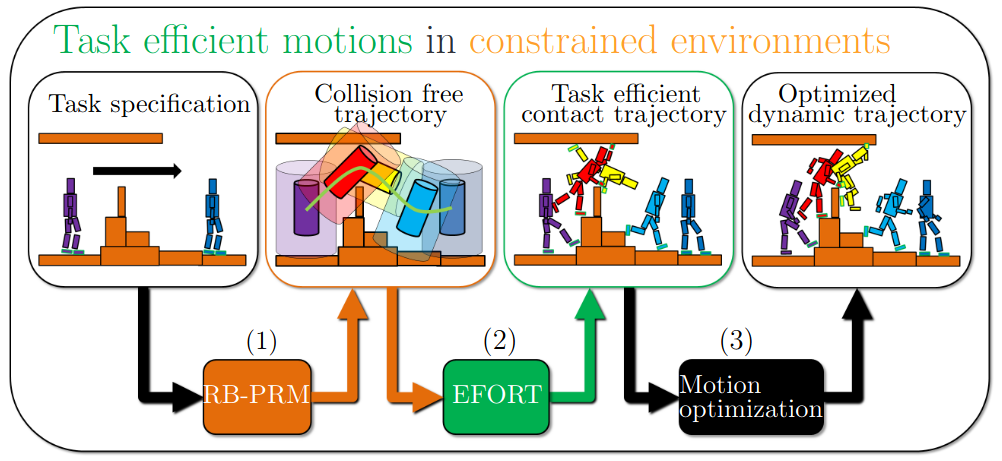
\includegraphics[width=0.8\textwidth]{Figures/Chapter_SOTA//diagram_steve_thesis.png}
    \caption{Motion-before-contact strategy, planning a rough robot trajectory to guide the contact planning. Source: Tonneau \cite{thesis_steve}.}
    \label{fig:cp_mbc}
\end{figure}

Planning only a few steps ahead requires the careful guidance of the robot to avoid falling into local minima.
On the other hand, planning several steps is subject to combinatorics, making the problem exponentially expensive to compute.

Inspired by some previous works on character animation \cite{thesis_kuffner_1999, pettre_2_stages_2003}, the motion-before-contact strategy alleviates these limitations by adding a higher-level planning layer, thus further dividing the contact planning problem into two modules (See (1) and (2) in Figure \ref{fig:cp_mbc}):
\begin{enumerate}
    \item A guide path planner, to generate a rough trajectory the robot has to follow to go through the environment (e.g. a robot base collision-free trajectory).
    \item A contact planner, to compute the contacts along this trajectory.
\end{enumerate}
Previously presented contact planners can thus be adapted to use a guide path to constrain the search for feasible contacts in the environment, and to obtain additional information about the path to traverse.


\paragraph{Guiding a contact planner.}
\begin{figure}[ht]
    \centering
    \captionsetup[subfigure]{justification=centering}
    \begin{subfigure}[t]{0.48\linewidth}
    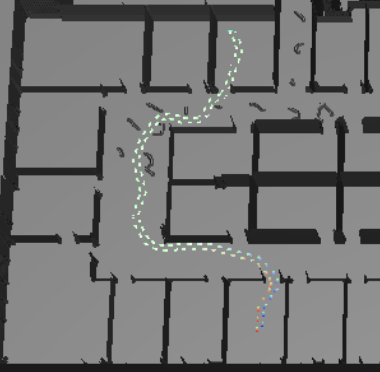
\includegraphics[width=\textwidth,height=4.5cm]{Figures/Chapter_SOTA//chestnutt_2004.png}
    \caption{Chestnutt et al. \cite{chestnutt_tiered_planning_2004}}
    \label{fig:cp_mbc_works_0}
    \end{subfigure}
    \begin{subfigure}[t]{0.48\linewidth}
    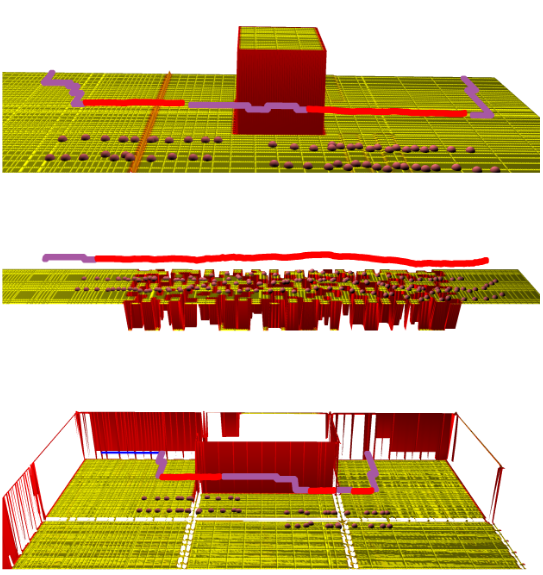
\includegraphics[width=\textwidth,height=4.5cm]{Figures/Chapter_SOTA//brandao_traversability.png}
    \caption{Brandao et al. \cite{brandao_multimode_2019}}
    \label{fig:cp_mbc_works_1}
    \end{subfigure}
    \caption{Examples of work on motion-before-contact planning.}
\end{figure}
Planning a robot trajectory is a problem of lower complexity that can be used for both horizons of contact planning.
Using a guide to control the input direction of short horizon footstep planners, can potentially solve their local minima issue \cite{norby_skd_2022}. 
On long horizon planners, the guide can constrain the search for footsteps around the guide, thus alleviating the combinatorics of the problem \cite{Hildebrandt_lola_2017}.

Using this architecture, Chestnutt et al. first manually define a graph searched for a 2D collision-free path \cite{chestnutt_tiered_planning_2004, Chestnutt2007NavigationPF} (Figure \ref{fig:cp_mbc_works_0}) or interactively drawing it on a user interface \cite{chestnutt_2009_interactive_guide}. This path then guides an A*-based contact planner.
Similarly, Yoshida et al. \cite{yoshida_2005} introduce a guide planner using a bounding box to model the robot moving while manipulating a large object. Their method generates collision-free trajectories to go through the environment, then followed by a pattern generator.

These works have been extended to more complex terrains with a reachability condition to plan 3D guide paths, before computing a sequence of contacts along it \cite{RB-PRM, AcyclicCP, rough_terrain_reachability_hutter_2021}.
% This condition is used in a sampling-based path planning algorithm, 
Using this condition, guide paths can also help in solving the surface selection problem of continuous contact planning methods \cite{sl1m_v2}.
In a model predictive control fashion, Risbourg et al. \cite{fanny_mip_solo} 
use a guide to obtain candidate contact surfaces and allow real-time short horizon footstep planning with a MIP method on the quadruped Solo.

Motion-before-contact approaches have proven successful in efficiently planning contacts for legged character locomotion \cite{egges_2010, bouyarmane_2009, bouyarmane2018}.
However, it also presents some limitations as explained in \cite{escande_2008}, where the guide should be rough enough to be quickly planned while being constrained enough to generate feasible contacts along.


\paragraph{Estimating the traversability.}
Planning a path according to an estimation of the difficulty to traverse the terrain can generate guide paths more likely to be feasible by contact planners.
This strategy has been used to move some quadruped robots through difficult rough environments \cite{kolter_2008, terrain_map_mrinal_2011, winkler_2014, winkler_carlos_2015, wermelinger_2016}. 

% Lin 2018/2021 (traversability)
% Brandao et Havoutis 2019/2020 same
Additionally, the guide paths can give information about the sections of the terrain traversed, permitting different walking strategies in function of its difficulty, also known as the multi-modal planning problem.
To move a humanoid robot in cluttered environments, Lin et al. \cite{lin_traversability_2018} plan a torso guide path using an A* searching algorithm on a cost map, and accounting for the difficulty of traversing the environment. 
They then decompose the guide path into segments, selecting for each one a locomotion mode. They switch between simple biped walking on flat ground or multi-contact locomotion using the robot's hand for increased stability in cluttered environments.
In the same line of work, Brandao et al. \cite{brandao_multimode_2019} use a quadruped robot body path to plan the different modes, such as a walking or trotting gait on flat ground, and contact planning on terrains requiring careful footstep placements.
Their results demonstrate that multi-modal planning locomotion can potentially achieve faster computation speed than pure footstep planning methods.

% Mini-conclusion: Such approximation considerably improve the computation time by lowering the complexity of the problem, where the goal is just to compute contacts along the collision-free guide given in input.
% Previous works were using it just to avoid collision, but the notion of reachability introduced by steve or carlos (?) is promising for the motion-before-contact strategy.
% Some works also uses the guide in different way: follow exactly the guide to compute the contacts, use the guide only to compute the contacts and ditch it after, use it to prune the surfaces, or use it in the notion of traversability to for multi-modes.
\paragraph{Conclusion on motion-before-contact.}

The motion-before-contact strategy is promising toward faster contact planning for legged robot locomotion.
% I WILL TALK ABOUT IT IN THE NEXT SECTION
%Different methods to generate the guide path have emerged using height maps, grids, or graphs solving a \textit{Navigation task}.
A prior guide path can be used in different ways by contact planners. 
Some works use it to accelerate the search for footsteps around the guide path, while others use it to get information about the traversed terrain to also solve the multi-modal planning problem.

%However, the benefits of this approach also comes at the cost of the non-guarantee of the path feasibility by the contact planner.
%That is why, previous works typically use heuristics to approximate the feasibility of the contact planner considered during guide path planning.
%These methods will be further covered in the next section on legged navigation.

% Modif par nicolas
The key aspect of motion-before-contact is the question of feasibility. If the feasibility is properly captured, then we can hope to quickly plan good guide paths before selecting contacts. Otherwise, the trade-off between planning infeasible paths or missing valid sequences will certainly lead to an over-conservative planner, with strong practical limitations.

So far, properly describing the feasibility with generic models has been the main bottleneck to these approaches, as we will see in Section \ref{subsub:nav:legged}.


\subsection{Conclusion}

% In a hierarchical decomposition of locomotion tasks, contact planning is usually done as contact-before-motion. While a step by step planning is possible, this can lead to local minima on more complex terrains and that is why we often want to plan several footsteps ahead to walk. But this brings a combinatorial aspect to the problem that can lead to high computation time >1s.

% COMMENTED
%Contact planning is a classical low complexity approach to solve the locomotion problem. The contact-before-motion strategy has been widely used in robotics to plan feasible footsteps in complex environments. Short horizon planning is fast to compute, but can be prone to local minima. Inversely, long horizon planning allows to ensure the completeness of the problem, at the cost of a higher computation time, where the inherent combinatorics of the problem has to be solved using discrete or continuous methods, and can lead to exponential computation times in function of the size of the problem.

% COMMENTED
%To alleviate these limitations, the motion-before-contact strategy proposes to plan a rough robot path in the environment prior to the contact planning phase. Using a high-level path is promising to guide or constrain the search for footsteps, while getting some information about the terrain to adopt the best walking strategy. The motion-before-contact approach has the potential to alleviate the limitation of current contact planner, that are the combinatorics or the local minima. Thus, it is a promising strategy for interactive replanning. However, using a guide also raises the problem of the non-guaranteed feasibility of the guide path with the contact planners. 

% COMMENTED
%Finally, generating a guide path introduces a new dimension to the locomotion problem that has been widely studied in other fields of the literature: the \textit{navigation} task.

% COMMENT NICOLAS: mieux articuler la conclu
% 1 - contact planning is yet a needed stage when generating complex movements.
% 2 - It relies in general to specific/adhoc model reduction combined to dedicated algorithms to explicitely tackle the discrete nature of contact sequences.
% 3 - We prefer MBC, because CBM leads to untractable complexity.
% 4 - MBC in turns implies guide planning, also separately handled as legged navigation.

Contact planning is yet a needed stage to generate, in tractable time, complex movement on legged robots.
This task relies on specific model reduction, to ensure footsteps feasibility, that is combined with dedicated algorithms to tackle the discrete nature of finding contact sequences.

In this section, we categorized contact planners into two categories.
The \textit{contact-before-motion} approach can lead to local minima on short horizon planning, and become computationally intractable on a long horizon.
That is why our research will focus on \textit{motion-before-contact}, that is promising to alleviate these limitations.
However, it raises the problem of the non-guaranteed feasibility of the guide path by a given contact planner.
The motion-before-contact approach in turn implies guide planning, that can be separately handled as a legged navigation task.


%About these walking strategies, an interrogation we would like to raise and that has not been totally answered is: \textit{Is there a real benefits for longer horizon over short horizon contact planning in most scenarios ?}
%In the context of the free-climbing problem \cite{bretl2006}, it is trivial to solve the combinatorics to find the optimal sequence of contacts. 
%However in the context of legged-locomotion, knowing that a feasible guide exist to move through the terrain, recent works on short horizon planner \cite{fanny_mip_solo, hutter_last_work_nmpc} could already lead to impressive results, removing this combinatorial aspect. \textcolor{blue}{False, to change}
%This question deserves further discussion in the future.

% On the other hand motion-before-contact, with the use of rough body path is promising to alleviate or break this combinatorics, constraining the exploration on a smaller region, prior to a contact planner computing the footsteps along it. 
% From guide path generated by the user or other navigation methods, this strategy has given impressive results with high computation time under a second on the vast majority of these works.
% However this additional hierarchical decomposition leads to a problem : It reduces the number of available solutions and thus, increases the risk to not finding a feasible contact sequence along the guide. (See citation bellow)
% In other words, we have no guarantee that the guide path is feasible by the contact planner.

% Chestnutt: "This is more computationally expensive than solving them separately, but ensures that the planner does not commit to a torso path that is unexecutable."
% "building a good approximation of the cost of reaching one torso position from another is extremely difficult compared to reasoning about the connectivity of stances"
% “difficult to efficiently guarantee that a particular torso path can indeed be followed by the robot (...) reasoning about foot contacts, it is much easier to provide guarantees of executability”

% Zucker says about contact-before-motion: "[ours] is capable of walking over a wider range of terrains, because the body path planner [others] at the most abstract level (...) is too conservative relative to the full range of possible footholds"

% Perrin says: “a high level planner might miss existing solutions that would have been found by the lower level planner”. + Discussion of Escande 2008 about it


\section{Navigation Task \label{sota3}}

\begin{figure}[h]
    \centering
    \captionsetup[subfigure]{justification=centering}
    \begin{subfigure}[t]{0.40\linewidth}
    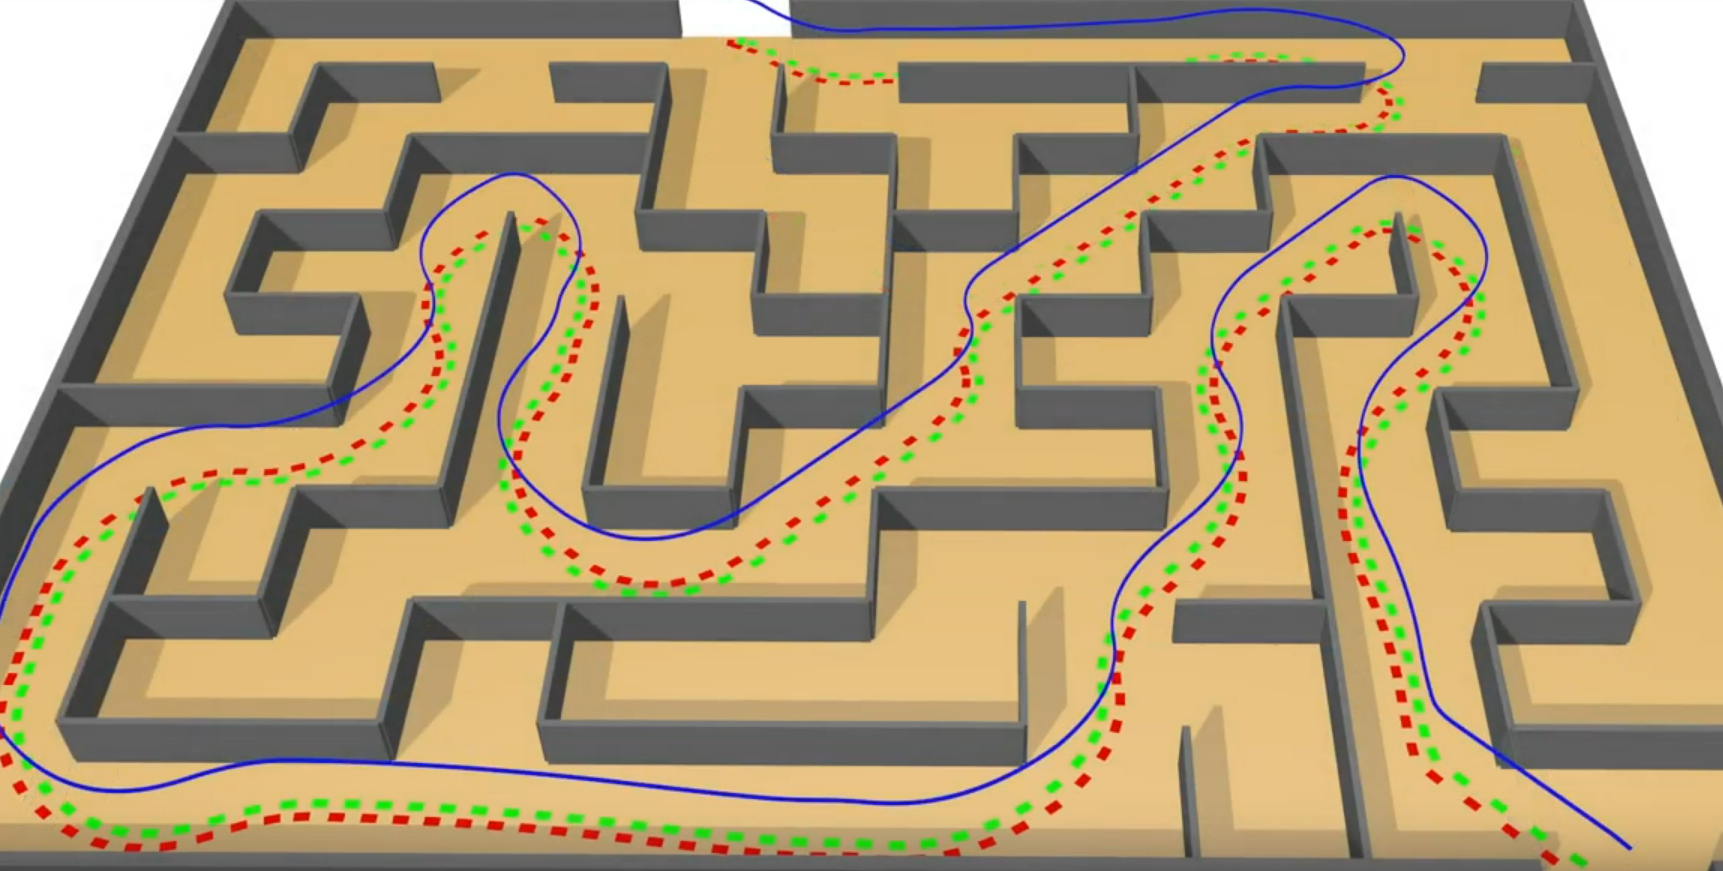
\includegraphics[width=\textwidth,height=4cm]{Figures/Chapter_SOTA//sl1m_maze.png}
    \caption{Global planner}
    \label{fig:nav_ex_0}
    \end{subfigure}
    \begin{subfigure}[t]{0.40\linewidth}
    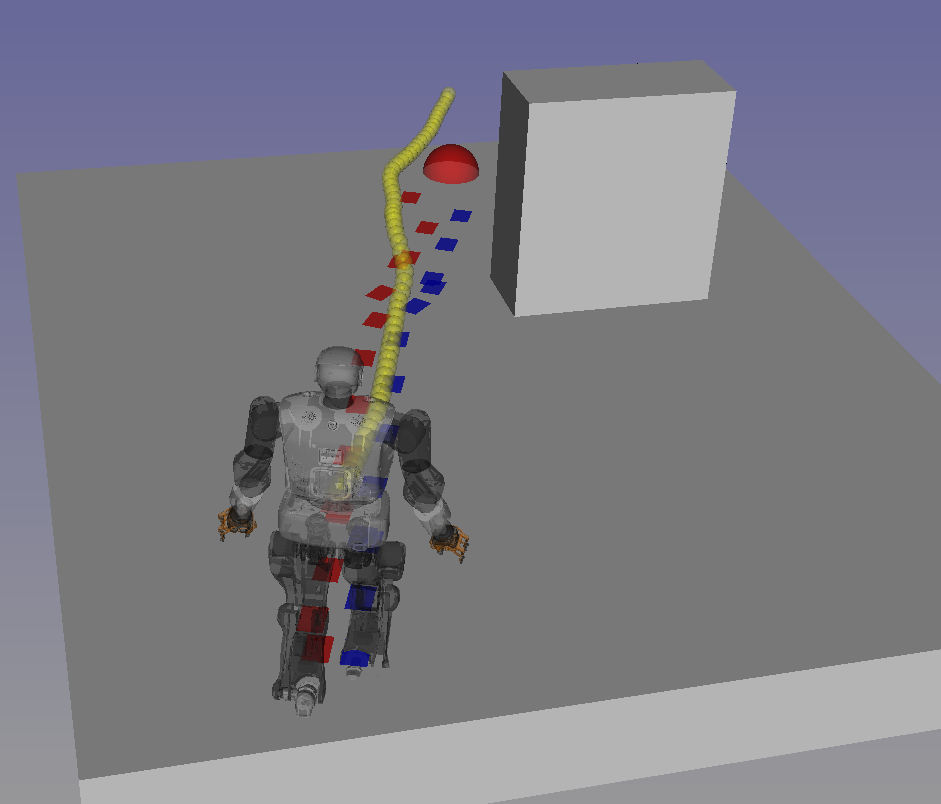
\includegraphics[width=\textwidth,height=4cm,trim={2cm 2cm 2cm 0},clip]{Figures/Chapter_SOTA//local_planning_wall.png}
    \caption{Local planner}
    \label{fig:nav_ex_1}
    \end{subfigure}
    %\label{fig:nav_ex}
    %\begin{subfigure}[t]{0.4\linewidth}
    %includegraphics[width=\textwidth,height=4.5cm]{Figures/Chapter_SOTA//dwa_rl.png}
    %\caption{Patel et al. \cite{patel_dwa_rl_2021}}
    %\label{fig:nav_ex_1}
    %end{subfigure}
    \caption{Navigation task at two different scales. Sources: (a) Tonneau et al. \cite{sl1m_v1}, and (b) a simulation in HPP \cite{HPP}.}
\end{figure}


Navigation can be formulated as the problem of planning and following a conflict-free path from some initial to goal positions, where conflict-free refers to the satisfaction of validity criteria (e.g. collision-free).
This challenging task has been extensively studied in the context of legged system or various autonomous vehicle navigation.
In particular, the environments they move in are often partially known or dynamic, thus requiring fast planning while satisfying optimality criteria.

To solve this problem, the navigation task can be performed with different architectures operating at different scales \cite{review_autonomous_2011}. 
Recent state-of-the-art implementations for autonomous vehicles, like the ROS navigation stack for 2D navigation \cite{ROS_software}, or for crowd simulation \cite{vantoll_microscopic_crowd_2021} employ an architecture composed of two modules:
\begin{itemize}
    \item Global planner, that plans a rough feasible path through the environment to a goal (Figure \ref{fig:nav_ex_0}). This is usually performed by \textit{path planning} algorithms that search for sub-goals to reach sequentially with a local planner.
    \item Local planner, that follows the rough path under specified rules. These rules can for example be based on the current sensory information of the robot for collision avoidance (Figure \ref{fig:nav_ex_1}). 
    This is usually performed by \textit{motion planning} (or \textit{trajectory planning}) algorithms that consider the robot or vehicle dynamics. Here, we will call such a local planner a \textit{steering method}, which is a widely used term in navigation.
\end{itemize}

%Section \ref{subsub:nav:overview} has a pedagogic purpose, in which we will present generic algorithms for both global and local navigation. Finally, we refer the reader to Section \ref{subsub:nav:legged} for the use of these algorithms in the context of legged robot navigation.

The contribution specific to legged navigation is mostly in the definition of the steering method, whose main challenge is to capture the feasibility of the robot whole-body, hence leading to acceptable robust or even natural movements. Yet, the properties that one must aim for when designing a steering method cannot be understood without, first, the algorithms underlying the navigation problem.
While we expect most of our readers to be already familiar with these algorithms, we decided to dedicate the next Section \ref{subsub:nav:overview} to a tutorial about them. Expert readers can skip it. Then we explore the existing contributions specifically addressing
the legged navigation problem in Section \ref{subsub:nav:legged}. This will enable us to finally give my thesis contribution as a conclusion to this chapter.


\subsection{Overview: Navigation Methods\label{subsub:nav:overview}}
We propose to explore the algorithms used in the broad context of navigation.
These algorithms can be categorized depending on the scale they operate in.

\paragraph{Global navigation in known environments.}\mbox{}\\

Consider a complex environment in which the robot has to move from an initial to a goal configuration.
By knowing the full model of the terrain in 2D or 3D, various strategies have emerged to solve the path planning problem.

We will explore the two main strategies for path planning that are \textit{graph-based} and \textit{sampling-based}.
These methods were previously introduced to solve the discrete contact planning problem (Section \ref{subsub:contact-before-motion}).
%and to solve a navigation task in the context of motion-before-contact strategy. 
Here we will present these path planning algorithms for a wide range of navigation applications.
Due to the global scale they operate on, most path planning algorithms do not consider the kinetics and kinodynamics of the system (e.g. maximum acceleration, velocity, and steering angle). 
Indeed it would result in burdensome computation time. 
That is why these constraints are often considered by the local planners that will be presented in the next section.\\

\noindent\textbf{Graph-based searching.}
% Read : Indicative Routes for Path Planning and Crowd Simulation, that explain very well all that.
% Say that from a graph, we have efficient algo to search it, mainly djikstra then A* and all its variations.
A graph is a structure composed of nodes and links, that are the discretized robot or character positions and their connections to other nodes respectively.
This graph is then processed by a search algorithm that solves a combinatorial problem to find the shortest path from the initial to the goal configurations. 
These search algorithms have a long history in the path planning field with Depth-First Search, Breadth-First and the well-known Dijkstra algorithm \cite{dijkstra_1959}. 
%These search algorithms have a long history in the path planning field with Depth-First Search, Breadth-First and the well-known Dijkstra algorithm \cite{dijkstra_1959}. 
%The latest uniformly explores the links according to their cost (e.g. path length) and selects the optimal path up to the goal. % (i.e. with the lowest sum of cost)
%A limitation of this uniform exploration strategy is that it can result in high computation time on long paths or in more complex environments.
Numerous search algorithms emerged to more efficiently explore such graphs, among which A* \cite{A_star_1968}, biasing the exploration toward the objective, along with its variants D* \cite{D_star_1994}, for an efficient replanning on unknown or partially known environments, or Anytime Repairing A* (ARA*) \cite{ara_star_2003} finding a suboptimal solution quickly then optimized toward optimality.

Now that we know efficient algorithms exist to search a graph, we are left with the question: \textit{How to build such a graph?}
% Predefined graph "waypoint graphs" => Not much to say here.
Manually specifying each node and link (waypoint graph) is a possibility to ensure the construction of a graph with conflict-free links \cite{waypoints_graph_lars_2002}.%, Chestnutt2003}. 
However, more generic methods requiring less cumbersome manual labor are preferred, such as Voronoi diagrams \cite{voronoi_example_2007} or visibility graphs \cite{visiblity_graph_example_2004}. \\
%\textcolor{blue}{I talk about it, but I do not explain them, it's long enough like that. How to say that I won't explain it here ?}

\begin{figure}[h]
    \centering
    \captionsetup[subfigure]{justification=centering}
    \begin{subfigure}[t]{0.4\linewidth}
    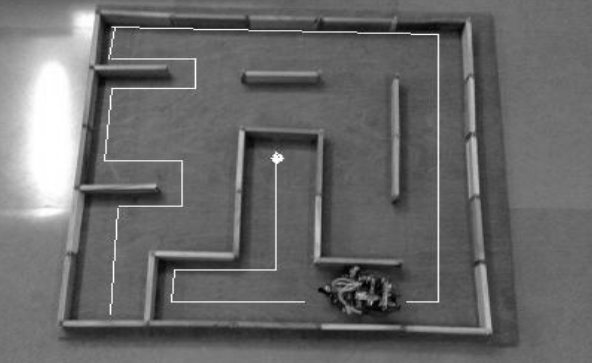
\includegraphics[width=\textwidth,height=3.5cm]{Figures/Chapter_SOTA//micromouse_maze.png}
    \caption{Micromouse challenge}
    \label{fig:global_nav_0}
    \end{subfigure}
    \begin{subfigure}[t]{0.4\linewidth}
    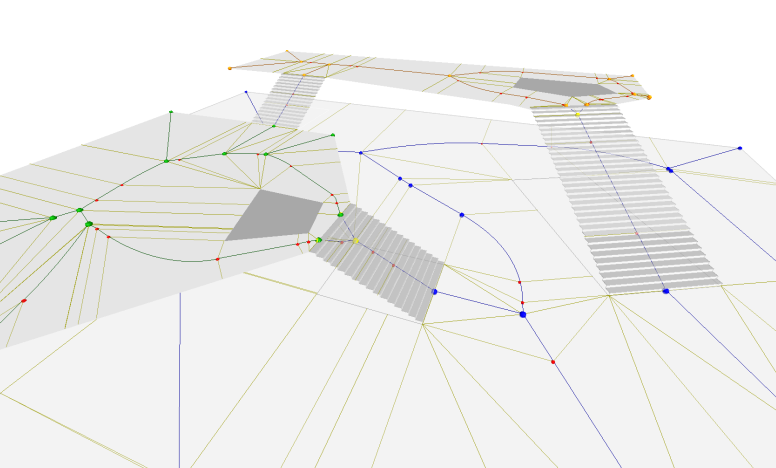
\includegraphics[width=\textwidth,height=3.5cm]{Figures/Chapter_SOTA//navMesh.png}
    \caption{NavMesh}
    \label{fig:global_nav_1}
    \end{subfigure}
    %\begin{subfigure}[t]{0.32\linewidth}
    %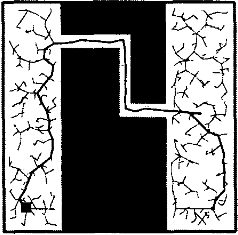
\includegraphics[width=\textwidth,height=3.5cm]{Figures/Chapter_SOTA//rrt_connect.png}
    %\caption{RRT-connect}
    %\label{fig:global_nav_2}
    %\end{subfigure}
    \caption{Examples of global navigation in 2D and 3D, sources: (a) Mishra et al. \cite{micromouse_mishra_2008}, (b) Toll et al. \cite{toll_2011_navMesh}} %and (c) Palmieri et al. \cite{RRT_distance_palmeieri_2015} }
    \label{fig:global_nav}
\end{figure}

\noindent\textbf{Grid discretization.}
% Grid => Most the works => % Definition of gried in Philippsen 2005 is ok.
Grids are used to uniformly decompose the environment into cells. 
Each cell corresponds to a node in the graph that is linked to its adjacent neighbors in free space (i.e. not occupied by any obstacle), thus forming a graph covering the full environment on which we use a search algorithm.
% ROS is using 2D grid was well to plan a global path
ROS navigation stack \cite{ROS_software} models the environment as a grid, which is then used for global path planning on mobile robots. The grid can represent an occupancy map indicating the presence of obstacles, or a cost map indicating the difficulty to traverse each cell.
% Path Planning with Modified a Star Algorithm for a Mobile Robot (Duchon 2014)
Several searching algorithms have been introduced for navigation in grid environments, mostly developing variants of A* algorithms to improve the computation time and optimality of the paths \cite{Philippsen_2005, grid_duchon_2014}.
% Micromouse will flood fill
In the Micromouse challenge, where a mouse robot has to explore a maze and then build an optimal path up to the goal (Figure \ref{fig:global_nav_0}), modeling the maze as a grid and planning the shortest path with a flood fill algorithms has been one of the most successful strategy \cite{micromouse_mishra_2008, micromouse_Benavides2018}.
% Integrated path planning and dynamic steering control for autonomous vehicles (Thrope 1986)
%Using a two-level architecture, Krogh et al. \cite{krogh_1986} first compute waypoints on a globally desirable trajectory, then use a local planner to generate conflict-free trajectories in between waypoints.

% Mini conclu on grid
Representing the environment as a grid is a simple yet efficient strategy to compute global 2D paths for various vehicles \cite{car_grid_ferguson_2008, singh_boat_grid_2018, saeed_grid_2020}.
In the same manner, grid decomposition can be extended to 3D using voxels \cite{3d_field_voxel_carsten_2006, uav_aerial_perez_grau_voxel_2017}. However, it raises the dimension of the problem, which can lead to intractable complexity.\\


\noindent\textbf{Navigation meshes.}
% Navigation meshes
These methods also called NavMesh \cite{navMesh_book_snook_2000} have long been used in the video game industry \cite{Brewer2019TacticalPO} and crowd simulation \cite{van_toll_crowd_sim_2012} to move some simulated characters. 
They use the terrain geometry, grids or voxels to decompose it into convex polygons traversable by a character. From the polygons, we can then generate a graph of conflict-free links (Figure \ref{fig:global_nav_1}).
% Gait mesh + Papers of Geraerts
Toll et al. \cite{toll_2011_navMesh, toll_2018_navMesh_multiLayer} compute navigation meshes in the order of milliseconds using their method, then search it to efficiently plan paths for thousands of virtual characters in real-time.
%However, the resulting set of paths can be limited in terms of possibility and require further editing \cite{sketch_navmesh_montana_2019}.
However, it requires a full model of the environment as well as an offline preprocessing phase to build the mesh.
Navigation meshes can be a computationally efficient solution for interactive global navigation, depending on the model of the scene and the NavMesh method used \cite{pettre_comparative_navMesh_2016}.\\


\noindent\textbf{Sampling-based algorithms.\label{subsubpar:sampling_based_algo}}
% Read kris hauser : https://motion.cs.illinois.edu/RoboticSystems/MotionPlanningHigherDimensions.html
Building graphs for navigation in a higher dimension or very large terrains can become intractable, as the combinatorics exponentially increases with the size of the search space \cite{hauser_robotics_systems_draft}.
In these cases, sampling-based strategies such as Probabilistic Road Map (PRM) \cite{prm_1996} and Rapidly-exploring Random Tree (RRT) \cite{RRT_1998} are particularly efficient to build a graph or a tree respectively.

Sampling-based algorithms have been widely used for navigation, using PRM \cite{move3d_lamiraux_2001, sabo_aerial_fuzzy_2012, mohanta_prm_navigation_2019} and RRT \cite{Zammit2018ComparisonBA} as well as their variants.
The system dynamics can also be considered in the sampling, thus permitting motion planning.
However, it increases the problem dimension, and so the number of samples required and the planning complexity.
As a result, the efficiency of these algorithms boils down to their sampling strategy, and their local planner capabilities to generate link trajectories \cite{kinodynamic_sm_2017, prm_rl_2019}.\\

%While those algorithms can bias their random sampling to efficiently cover the search space, it is important to note that PRM and RRT both plan a feasible path to the goal and do not consider the optimality of the solution thus often resulting in jerky paths.
%Several variants of these algorithms exist to alleviate their limitations by performing a post-processing phase, but those will not be covered in this state of the art. 
%optimization on the feasible path toward optimality, but those will not be covered in this state of the art.


\noindent\textbf{Conclusion on global navigation task.}
A large panel of algorithms solves the global navigation problem \cite{motion_planning_latombe_1991, planning_algo_lavalle_2006, hauser_robotics_systems_draft}.
As it can be difficult to find which algorithm suits our application, several surveys exist to guide our choice \cite{yang_3D_path_planning_2016, Zammit2018ComparisonBA, patle_nav_mobile_robot_2019}.

Overall, global planners have to demonstrate efficient exploration capabilities of the search space.
Due to the scale they operate in, they often require an expensive offline phase to build the graph or searching time.
As a consequence, those are not suited for replanning in uncertain environments, where the global perception is rarely realistic and unexcepted events can occur.

That is why, it is preferred to combine these global algorithms with a simple linear interpolation to generate collision-free trajectories between graph nodes at a minimal cost, without considering the system dynamics. 
The graph is then searched to get a rough path (i.e. waypoints to reach sequentially), that is then followed by a local planner to handle environment uncertainty.



\paragraph{Local Navigation for environment uncertainty\label{subsub:nav:local}}\mbox{}\\

%\stn{donner l algo et ou une figure ça simplifierait la comprehension}

A local planner computes a trajectory between two points generated by a global planner.
In the context of navigation, we call such a local planner a \textit{steering method} (Figure \ref{fig:local_nav}). 
%It guides the trajectory toward a distant objective or its direction.
These local planners have been extensively used in navigation tasks for fast and local replanning.
Contrary to global planners, steering methods often do not require a guarantee of completeness or optimality but need to produce local paths under desired criteria, such as fast computation, collision-avoidance behavior, or kinetic and kinodynamic constraints.\\


\noindent\textbf{Definition of a steering method.}
The definition of the word \textit{steering} is \qq{the control of a vehicle to make it follow a route or direction}.
However, we identify in previous works different definitions for the term \qq{steering method}.

The first definition states that a steering method \qq{computes an open-loop trajectory that brings a nonholonomic system from an initial state to a goal state without the presence of obstacles} \cite{randomized_kino_planning_lavalle_2001}. 
This definition has been used in other works \cite{DIMT, move3d_lamiraux_2001} specifying that such steering methods exactly connect two states.

A broader definition is a local planner that \qq{follows the rough path while adhering to certain local rules} (e.g. collision-avoidance) \cite{van_toll_crowd_sim_2012}. 
Adherence to these rules can imply some reactive behaviors from observations of the terrain such as the presence of obstacles. % Pas obligatoirement
This definition is used in navigation \cite{ondrej_pettre_steering_vision_2010,prm_rl_2019} where the characters or vehicles are often steered toward waypoints obtained by global path planning algorithms, but may not reach them exactly. 
In this thesis, we will use the broader definition that we deem more relevant in the context of legged robot navigation.\\


\noindent\textbf{Terrain-free steering methods.}
Computing a trajectory connecting exactly two points without considering the environment can be done efficiently with model-based approaches.

% Interpolation techniques
% Linear interpolation
% Curves
Interpolation methods consist in computing a curve passing exactly through all the given sub-goals \cite{interpolation_methods_bourke_1999}. Linear interpolation is the simplest and fastest way to link two configurations in space, making it the default steering method of most graph-based and sampling-based algorithms, %and has been widely used in the context of legged robot navigation \cite{rough_terrain_reachability_hutter_2021, AcyclicCP}. 

% Trajectory optimizers as DIMT
Other interpolation methods such as bezier, spline, and hermite curves exist to obtain smooth and continuous trajectories.
Those curves can be a solution to perform motion planning, which regroups different terms as kinodynamic \cite{randomized_kino_planning_lavalle_2001, DIMT} or nonholonomic planning, that must account for constraints on the system dynamics (i.e. velocity and acceleration ) or whose state depends on the path taken respectively.
%Kinodynamic steering methods have seen some success combined with PRM \cite{florent_motion_planning_car_2001} or 
%RRT global planners . 
%One of these kinodynamic planners is the double-integrator minimum time, that has been used for planning on robot manipulators \cite{DIMT}. 
%This method has also been used to plan guide paths in the context of the navigation of humanoid robots \cite{kinodynamic_sm_2017} which will be used for comparisons throughout this thesis.

These steering methods exactly connect two sub-goals and are fast to compute as they ignore obstacles.
However, they heavily rely on conflict checking by the global planner when applied to complex environments. 
This can often be burdensome in algorithms such as PRM and limit their use in applications with environmental uncertainty which requires fast local replanning.\\

\begin{figure}[h]
    \centering
    \captionsetup[subfigure]{justification=centering}
    \begin{subfigure}[t]{0.4\linewidth}
    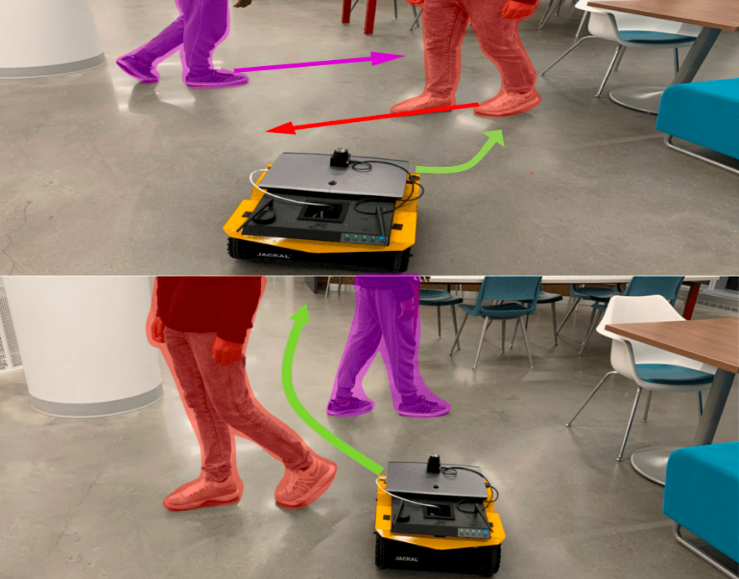
\includegraphics[width=\textwidth,height=4.5cm]{Figures/Chapter_SOTA//dwa_rl.png}
    \caption{Patel et al. \cite{patel_dwa_rl_2021}}
    \label{fig:local_nav_0}
    \end{subfigure}
    \begin{subfigure}[t]{0.5\linewidth}
    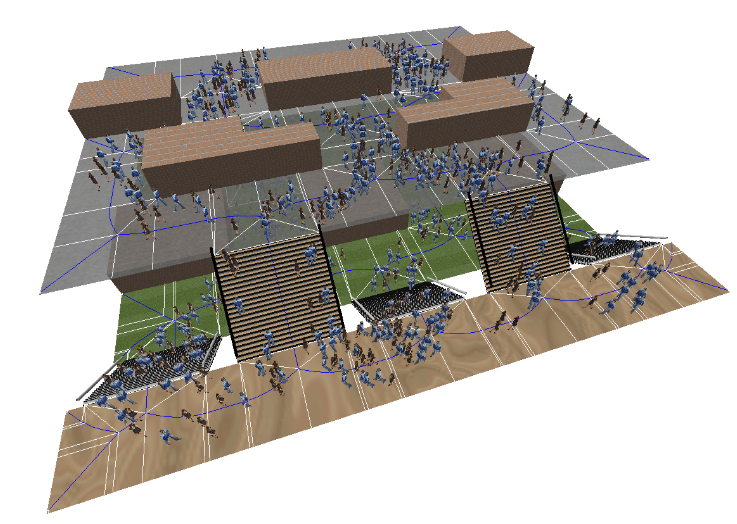
\includegraphics[width=\textwidth,height=4.5cm]{Figures/Chapter_SOTA//real_time_density_geraerts.png}
    \caption{Toll et al. \cite{van_toll_crowd_sim_2012}}
    \label{fig:local_nav_1}
    \end{subfigure}
    \caption{Examples of terrain-aware local navigation: (a) a mobile robot and (b) characters in a crowd simulation locally avoiding collisions with the terrain and other people.}
    \label{fig:local_nav}
\end{figure}

\noindent\textbf{Terrain-aware model-based steering methods.}
Computing a conflict-free trajectory considering the environment is another steering strategy. 
Those additional conflict-free constraints permit a local replanning in function of the environment observations, at a higher computation cost compared to terrain-free steering methods.

% STOMP => Consider obstacles, but stochastic and derivative-free
Local planning can be posed as an optimal control problem \cite{optimal_control_path_planning}. 
Liu et al. \cite{liu_mpc_path_planning_2017} use a model predictive control to enforce collision avoidance with other vehicles in the context of autonomous driving.
Depending on the formulation of the problem and the constraints modeling the environment, these optimization methods can be an efficient solution for locally terrain-aware planning.

% Potential field => Used in Corridor map and Explicit Corridor
Potential field \cite{potential_field_1992} is a common technique for path planning using local information about the environment \cite{mpc_potential_field_car_2017}. 
This method sees the terrain as an energy potential landscape where obstacles will repulse the robot, while the goal attracts it.
While this method could be used for global planning, it is by nature prone to local minima and therefore more suited for local and reactive terrain-aware planning.
Potential field has seen some success in crowd simulation with the corridor map method \cite{corridor_geraerts_2007, explicit_corridors_2010}, computing first a global path to follow, then locally planning some collision-free paths according to a potential field.

Some of the most widely used local motion planner for collision-avoidance in vehicle navigation are the Dynamic-Window Approach (DWA) \cite{dynamic_window_fox_1997} and the Time-elastic-band \cite{elastic_band_2013}, both presenting their advantages \cite{dwa_vs_teb_2021_rosmann, dimitri_these_2021}, and implemented in the ROS navigation stack \cite{ROS_software}.
% DWA (dieter 1997) => Does consider the terrain and collisions etc.
Dynamic-Window Approach (DWA) \cite{dynamic_window_fox_1997} discretizes the control space of the robot to generate a set of candidate trajectories. 
The best trajectory is then selected based on a user-defined score (e.g. collision avoidance, clearance to obstacles, distance to goal). Those steps are performed continuously during the navigation and permit a fast replanning. However, this method can be computationally burdensome depending on the discretization of the control space, and the complexity of the conflict checking along the candidate trajectories.
% TEB
Time-elastic-band \cite{elastic_band_2013} optimizes a robot trajectory generated by a global planner. This trajectory can be seen as an elastic band that will be modified considering some objectives such as minimizing its path length or time, or obstacle avoidance.

% Velocity field => crowd sim multi char
% ORCA
The crowd simulation field has also developed methods for local collision-avoidance behaviors between autonomous agents and their environment. One of them is the Optimal Reciprocal Collision Avoidance (ORCA) algorithm \cite{orca_2011} selecting the best action to compute collision-free motions for thousands of characters in real-time (Figure \ref{fig:local_nav_1}). 
These methods solve a particular problem that is the collision-avoidance in highly dynamic environments, subject to different criteria (e.g. social distances or group behaviors). Those are not applied in the context of this thesis, but we refer the reader to the survey of Toll et al. \cite{vantoll_microscopic_crowd_2021} for further details.\\


\noindent\textbf{Terrain-aware RL steering methods.}
% MDP for discrete actions, possible on grid etc also. (see the book of hauser)
Reinforcement learning has seen a lot of success in locally terrain-aware navigation due to its perception and generalization capabilities, and robustness to uncertainty.

% Crowd simulation
Controlling an agent in velocity and orientation, RL controllers have been used for steering in crowd simulation \cite{survey_rl_animation_pettre_2022} and autonomous robot navigation \cite{collision_avoidance_rl_multiagent_chen_2016, survey_rl_driving_kiran_2020} in uncertain and dynamic environments.
Lee et al. \cite{jaedong_2018_crowd_rl} present a method to teach an agent collision avoidance behavior, using rays to detect obstacles and other agents.
Francis et al. \cite{prm_rl_2019} learn an RL steering control over linear and angular velocity on an autonomous mobile robot for local navigation. They also use this steering method inside a PRM to evaluate the links feasibility and build a graph.
%Multi-Agent RL (MARL) is an interesting approach to learn interactions between two characters. 
%Chen et al. \cite{collision_avoidance_rl_multiagent_chen_2016} present a decentralized multi-agent approach to learn collision avoidance by reinforcement on two mobile robots. Their results show that the learned policy can generate natural and smooth trajectories while avoiding other humans or virtual agents.
Combining RL with model-based approaches Patel et al. \cite{patel_dwa_rl_2021} generate trajectory candidates using the Dynamic Window Approach (DWA), then learn a policy to select the best candidate (Figure \ref{fig:local_nav_0}).
Finally, Muller et al. \cite{dwa_gan} use an evolutionary algorithm to generate candidate trajectories, thus potentially generating better motion plans than a classical DWA approach.

Different representations of the environment can be used to learn local planners such as velocity fields \cite{deep_multiagent_crowd_2020}, depth images \cite{learn_steer_2018}, lidar sensors information \cite{prm_rl_2019, RL_RRT} or occupancy grids \cite{rl_navigation_video_game_2020}.

Reinforcement learning is a powerful tool to achieve behaviors that are complex to engineer with model-based approaches.
In the context of local navigation, those methods tend to adapt well to uncertain or partially known environments.
They are a pertinent choice over model-based approaches to learn how to solve complex navigation tasks while respecting some desired criteria.\\
% We do not talk about evolutionary algorithms in this section that can be a suitable alternative to RL for navigation.
% Paper of deepmind: evolutionary vs rl + majid 2021
% Evolutionary-Group-Based Particle-Swarm-Optimized Fuzzy Controller With Application to Mobile-Robot Navigation in Unknown Environments


\noindent\textbf{Conclusion on local navigation.}
% Discussion on terrain-aware vs terrain-free
%We have seen two definitions of steering methods to locally compute a trajectory between two points. 
Terrain-free steering methods are fast to compute, but have to rely on expensive global planners for conflict checking and replanning when facing environmental uncertainty.

Terrain-aware methods can remove the need for replanning on simple scenarios by generating conflict-free paths. %, however resulting in higher computation times.
%They have been widely used to follow paths computed by global planners.
While model-based approaches can efficiently compute trajectories with collision-avoidance behaviors (e.g. ORCA, DWA), reinforcement learning is particularly promising to learn complex navigation tasks.
It is used in the context of autonomous mobile robot navigation to learn policies collision avoidance with humans, or crowd simulation to learn social distancing and adapting to other agents steering behavior. 
Furthermore, they can generalize well to unexpected events and partially known environments by using rich perceptual observations.




\subsection{Navigation Task for Legged Robot Locomotion\label{subsub:nav:legged}}
\begin{figure}[h]
    \centering
    \captionsetup[subfigure]{justification=centering}
    \begin{subfigure}[t]{0.40\linewidth}
    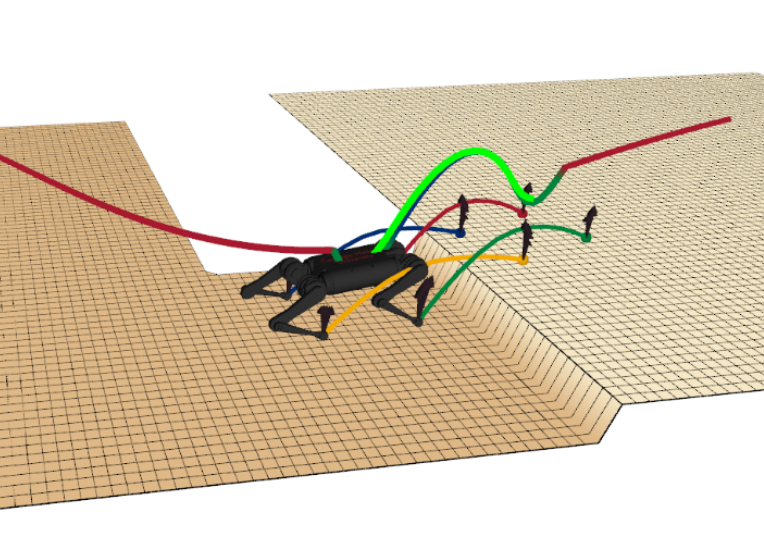
\includegraphics[width=\textwidth,height=4.5cm]{Figures/Chapter_SOTA//norby_2022.png}
    \caption{Norby et al. \cite{norby_skd_2022}}
    \label{fig:legged_nav_0}
    \end{subfigure}
    \begin{subfigure}[t]{0.40\linewidth}
    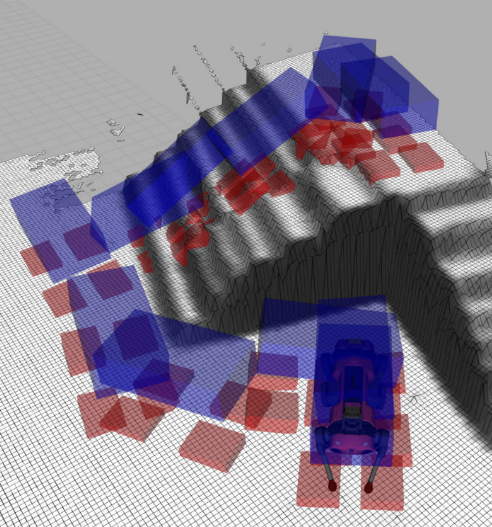
\includegraphics[width=\textwidth,height=4.5cm]{Figures/Chapter_SOTA//hutter_guide_path.png}
    \caption{Wellhausen et al. \cite{rough_terrain_reachability_hutter_2021}}
    \label{fig:legged_nav_1}
    \end{subfigure}
    \caption{Legged robot navigation for motion-before-contact planning.}
\end{figure}

%We now want to focus on the application of navigation algorithms for legged robot locomotion.

% Chestnutt 2003 => waypoint graph
%In the context of motion-before-contact, manually defining the guide path to follow is a solution for fixed scenarios \cite{Chestnutt2003}. However, automatizing their generation with a navigation algorithm is required to cover a larger panel of terrains \cite{darpa_hutter_2022}. The problem these planners have to solve is: \textit{How to generate a feasible guide path for the contact planner?}


Historically, navigation methods have been used on large near-flat terrains \cite{Chestnutt2007NavigationPF} or legged robots and avatars \cite{pettre_2_stages_2003}, paying mostly attention to naturalness \cite{isabelle_maroger_2020}. Yet, as soon as the environment is more constrained, legged navigation becomes a dedicated topic, with the central feasibility question: \textit{How can we plan a guide path while ensuring that a corresponding feasible whole-body trajectory exists?}
While no definitive answer yet exists, several advances have been made on a part of the problem main difficulties.


% === Conclusion on feasiblity of the guide by the CP ===
% Waypoint graph => they consider that it's good enough
% Grid => They consider that the heuristics score used to compute the guide is enough.
% Acyclic + hutter => They consider that the reachability condition is sufficient.
% Brandao => They trust their local planner (A*)

\paragraph{Collision-free path.}
%\textcolor{blue}{Nicolas: Titre a changer + "Section facile", il faut que je rajoute des papiers et expliquer plus en detail ce que j'entends par collision etc.}
Planning collision-free whole-body trajectories is required for legged robots to locomote through terrains with non-traversable obstacles.
Trivially, we have no access to these trajectories during navigation, but we can expect the robot base to be collision-free.

Following \cite{pettre_2_stages_2003}, previous works typically rely on simplified system walking models for collision detection such as collision boxes.
%that have long history in the character animation field for collision detection \cite{collision_box_1988}.
% Hildebrandt => 2D => Harmonic + time elastic band. Point model with a safe collision margin.
In \cite{Hildebrandt_lola_2017}, the robot is represented as a point with safe margins, simple yet efficient to generate 2D paths avoiding obstacles on flat terrains.
As a result, their footstep planner is guaranteed collision-free footstep trajectories, thus demonstrating clear computation gains over their previous contact-before-motion approach.
In \cite{rough_terrain_reachability_hutter_2021, lin_traversability_2018, AcyclicCP}, the robot torso is approximated by a simple box volume to significantly improve 3D collision checking speed, hence reducing guide planning time.

% Papier pettre: bounding box (pettre_2_stages_2003)
% Papier acyclic
% Papier hutter DARPA: darpa_hutter_2022 page 20.


\paragraph{Robot kinematic reachability.}
% Linear + PRM => Hutter + Acyclic
% Kinodynamic + RRT => Pierre + Norby 2020/2022
% NavMesh => brandao
Naturally, the extension of legged robot navigation to 3D also raises the question of reachability, where the robot should be kinematically able to reach the ground with its end effectors.
The reachability condition introduced by Tonneau et al. \cite{RB-PRM} use an approximation of the robot range of motion, that ensures the robot can reach the terrain all along the path. It has proven successful to generate guide paths on complex terrains with a high success rate for producing a sequence of whole-body posture. However, it turns out to be less successful when trying to connect these postures with feasible dynamic trajectories.

An approach is to incorporate these conditions in sampling-based path planning algorithms \cite{sl1m_v2}.
Some works use a PRM with a linear interpolation method \cite{AcyclicCP} for navigation and contact planning in tractable computation time, or RRT with model-based kinodynamic steering methods \cite{kinodynamic_sm_2017} for dynamic locomotion.
In this line of work, \cite{norby_2020} use a kinodynamic body path planner to guide their short-horizon contact planner. Their extended results show that their quadruped robot can walk and jump to locomote over complex terrains \cite{norby_skd_2022}(Figure \ref{fig:legged_nav_0}).

The reachability condition is the cornerstone to build legged robot contact planners.
%that go beyond simple obstacle avoidance behavior. 
Yet, it has limited performance as it implies hard-tuned heuristics models that are difficult to generalize, and often fail to capture the connectivity between successive key whole-body postures. %Supervised learning seems a direction to extend it, but the evident lack of dataset makes it difficult.


% Definition of traversability by yu-chin lin: Traversability is a measurement of how easy the contact space planner can generate contact sequences to traverse through a certain region.

\paragraph{Cost map for terrain traversability.}
As a refinement to these two required conditions, the fine details of the terrain map can be approximated by a so-called \textit{traversability} score, which evaluates how easy it is for the robot to traverse a region. This technic has been employed in particular during the DARPA challenge to locomote quadruped robots on rough terrains \cite{darpa_hutter_2022}. 

In \cite{kolter_2008, terrain_map_mrinal_2011, wermelinger_2016}, some hand-tuned heuristics are implemented to score footholds, hence evaluating how desirable a foot placement is at a given location. 
%This score is then used to compute the likelihood of a body position to find desirable and feasible contacts in complex environments.
% Grid => kolter / winkler / Arain 2013 / Wermelinger 2016
Following this approach, Winkler et al. \cite{winkler_2014} compute sequentially from a terrain height map: the footholds score map, then the corresponding body score map which evaluates the likelihood of a body position to find desirable and feasible contacts.
The body map is then searched to plan guide paths more likely to be feasible by their robot according to their heuristics.
However, these heuristics often require complex tuning to sufficiently approximate the robot capabilities, and result in expensive computation to build the map over the search space.
In \cite{lin_traversability_2017}, this last limitation is alleviated by learning regressors to estimate terrain traversability, faster to querry during planning. Their results demonstrate a higher contact planning success rate with their traversability estimation over a classical collision-free guide, but still at the cost of extra computation.

Combining terrain traversability with the reachability conditions, \cite{rough_terrain_reachability_hutter_2021} learn a foothold score predictor in a supervised fashion from a few manually labelled data. This predictor enables removing unsuitable geometry from the reachability space.
It is then proposed to employ the reachability condition with a PRM and linear interpolation to efficiently plan guides in complex terrains (Figure \ref{fig:legged_nav_1}).
By doing so, they ensure the presence of suitable surfaces to step on along the guide, hence potentially facilitating the robot locomotion with their blind controller \cite{hutter_challenging_terrain}.


Supervised learning seems a promising direction to learn how to approximate guide path feasibility by a contact planner and by extension the whole-body motion. 
Yet, they mostly rely on heuristics that are either too expensive to compute or can fail to sufficiently capture their capabilities.
Learning directly from these planners could solve these limitations, however, the evident lack of dataset makes it difficult to generalize.


%\textcolor{blue}{Nico: Trouver les arguments pour ca dans les papiers. Il faut que ca soit bien argumente pour dire que c'est pas assez. La conclu doit pouvoir etre percutante.}
%However, planning guide paths with a high traversability score is not yet sufficient to ensure contact planning success.
%Moreover, these methods require some computationally expensive offline and online phases, to build the cost map and search it respectively. 
%As a consequence, such a strategy is not yet tractable for real-time applications.

% Humanoid => Lin, he uses a cost-based grid as well. Explain specifically.
% It may not be useful to cite it here.



% What is the problem => On a plus la notion de traversabilité. Le terrain peut être atteignable oui, mais pas sûr qu'on puisse trouver une sequence de contact dessus.
%Previous works consider the reachability condition as being sufficient to approximate the feasibility of their contact planner. However, this condition may not be sufficient to generalize to the large panel of contact planning strategies. Moreover, this condition requires particular fine-tuning. Overestimating the robot range of motion can lead to unfeasible guide paths. Conversely, considering only a small range of motion can increase the guide success with a given contact planner, but also limit the guide planning navigation possibilities.




\subsection{Conclusion on Legged Navigation}
% Norby: The global planner is critical to this pipeline due to its place at the top of the planning stack. A good global planner must have an accurate idea of what the robot can and cannot do to ensure that the other layers can resolve the motion, but also must have a long enough horizon to avoid local minima which is difficult to achieve in real time. 

%In motion-before-contact, guide planning is critical due to its place at the top of the planning stack as stated by Norby et al. \cite{norby_skd_2022}. Such guide paths must take into account the robot capabilities, and ensure the success of the contact planning.

% Phrase par nico
Legged navigation is strongly related to motion-before-contact planning strategies. 
Solving it properly then turns the problem of finding a contact sequence to a much simpler one.
We follow the argument from Norby et al. \cite{norby_skd_2022} to consider it among the most promising directions to solve the contact planning problem.


A panel of strategies emerged to increase the success rate (or compatibility) of the guide with contact planners.
However, they either rely on often necessary but not sufficient conditions (e.g. collision-avoidance, reachability) or on heuristics to improve the likelihood of success that are computationally untractable.




% Talk about all navigation stuff and what exist => It's a jungle.
%Navigation at both global and local scales has been extensively studied for a wide variety of applications, ranging from autonomous vehicle navigation to crowd simulation.
% Talk about what is actually done in legged robots relatively to that
%In the context of legged robot locomotion and more specifically motion-before-contact approaches, these algorithms can be used to plan guide paths prior to contact planning.

% Very little works on guide feasibility. They conditions, then consider that it's ok.
% cost map for traversability is nice to improve the success rate but not tractable yet.
%Legged navigation methods have to solve the critical problem that is the feasibility of the guide path by a given contact planner.
%In spite of a few successes with heuristics, no work has yet fully addressed this problem in a tractable computation time.

%Most of previous works consider that collision-avoidance and reachability conditions along the guide.
%However, they are often not sufficient to ensure contact planning success.
%In the search for a general solution 
%Reinforcement learning has demonstrated impressive navigation 

% ================================================================


% However following the resulting rough global path with a terrain-aware steering method is better to consider the dynamic of the system and locally consider replanning for uncertainties in the environment. (corridor map do that for ex, or nav mesh)

% We did not explore all local and global planning strategies and focused on the one that could potentially be applied in this thesis for a character navigation task. More information can be found in the draft of Kris Hauser \cite{hauser_robotics_systems_draft} as well as the reference book in the topic \cite{Robot Motion Planning, planning_algo_lavalle_2006, }

%\section{General Conclusion \label{sota4}}
\section{What are the next steps in artificial locomotion? \label{sota4}}
% - General conclusion
%A division of the legged character locomotion problem is still required to interactively plan safe walking motions on complex terrains.
\subsection{Conclusion on legged locomotion strategies.}
%We have shown that, despite some recent promising approaches for legged character locomotion, agnostically considering the contact with the terrain to produce whole-body movement is yet unfeasible on real human-sized legged robots.
%We believe planning contacts and motion simultaneously to be the most promising solution to achieve this task in the future. However, this approach is yet computationally untractable.

Despite some recent promising approaches for legged character locomotion, there exists no locomotion solvers able to generate complex contact platterns without explicitely considering contact decisions on real humand-sized legged robots.
It seems evident to us that we must consider the whole problem of deciding contacts and motion simultaneously, both to formulate the theoritical objectives and in the perspective of a promising solution to achieve this task in the future.
However, tackling the whole problem in a unique motion solver is yet computationally untractable.

Dividing the locomotion problem in two parts, contact planning and whole-body control, is still required to plan safe robot locomotion in real time on complex terrains.
We explored the contact planning problem to automatically generate the contacts to be performed by the whole-body controllers.
We have seen contact planning at two different scales.
Short-horizon planning is fast to compute, but prone to local minima.
Long-horizon planning can offer some guarantee of completeness and potential optimality at the cost of a higher computation time.

% Motion-before-contact is promising to alleviate the limitation of both strategies.
% Explain the pipeline.
\textbf{Motion-before-contact} strategy is a promising solution to alleviate the limitations at both planning scales. 
This hierarchical approach contains the following modules:
\begin{enumerate}
    \item A \textbf{guide path planner} to plan a rough path the robot has to follow.
    \item A \textbf{contact planner} to plan the contacts along this path.
    \item A \textbf{whole-body controller} to compute the whole-body motion performing these contacts.
\end{enumerate}
We argued that this hierarchichal division offers the most promising directions. Yet, as in any divide-and-conquer approach, it raises the question of consistency in the hierarchy that we formulated as the \textbf{feasibility} question: \textit{How to generate feasible guide paths?}

The feasibility has been studied in several research fields. Yet we feel these tentatives lack of systematic approaches.
In particular, there is no proposed guarantee either theoritical or empirical that the propose feasibility conditions of one hierarchical level makes the resulting movement a valid guide for the following stage.
We propose to explore this problem with a reinforcement learning approach.
\textcolor{blue}{Nico a mis data-driven approach. En machine learning, data-driven veut dire qu'on utilise des bases de donnee. En RL ca veut dire qu'on entraine ou pre-entraine notre policy avec ces prior dataset, donc ce n'est pas le bon terme.}
\hfill \break
\hfill \break

The topic of this thesis is the integration of \textbf{legged navigation} in the decision flow of locomotion. Particularly, our first proposition is that the \textbf{feasibility condition} should be formulated in a way that intrinsically takes into account the limitations of the next task in the hierarchy, the \textbf{contact planning}.
We formulated our problem as follows: \textit{Can we plan feasible guide paths that are more likely to be extended into valid contact sequences?}

Previous works approach the problem by approximating the contact planner capabilities, such as the \textbf{reachability} condition \cite{RB-PRM} or other user-designed heuristics.
Then, they plan paths considering these approximations.
Arguably, they can often be insufficient or too complex to engineer depending on the contact planning strategy \cite{AcyclicCP, winkler_2014}.
But any such conditions so far has demonstrated strong practical limitations when scaling it to real scenarios (e.g. nicely producing valid contact sequences but failing to extend to complete dynamic trajectories). 
Our second proposition is to define dedicated feasibility conditions directly from data collected on past executions of the contact planner.
However, there is no evident existing dataset to start learning a feasibility condition, nor any method to compute sufficiently diverse paths and generate such data.
We then finally propose to approach the training of such a feasibility condition by \textit{Reinforcement Learning}. We learn the legged navigation task using the contact planner as an external oracle rewarding the navigation system for feasible guidance.

Our work find some inspiration in some recent works on reinforcement learning navigation \cite{prm_rl_2019, jaedong_2018_crowd_rl}. 
This thesis further explores this approach in the context of legged character locomotion.
We answer the question: \textit{How to learn by reinforcement a navigation task for a better contact planning feasibility?}

%Our work find some inspiration in recent works on Reinforcement learning for autonomous vehicle navigation \cite{prm_rl_2019} and crowd simulation \cite{jaedong_2018_crowd_rl}.
%In these works, RL agents can navigate using partial observations of the terrain and under complex constraints, that are often too difficult to handle with model-based approaches.
%We investigate this approach in the context of motion-before-contact, where reinforcement learning could be a computationally efficient solution to the guide path feasibility problem.